\documentclass[12pt]{article}  
% Alternative for A4: \documentclass[12pt,a4paper]{article}  

\usepackage{CSPArticleStyle}

% - - - - - - - - - - - - - - - - - - - - - - - -
% additional packages
% - - - - - - - - - - - - - - - - - - - - - - - -
\usepackage{csquotes}
\usepackage[margin=1in]{geometry}
\usepackage{xypic}
\usepackage{booktabs}
\usepackage{parskip}
\usepackage{amsmath}
% Font settings - Times New Roman  
\usepackage{times}  
\usepackage[T1]{fontenc}  
\usepackage[utf8]{inputenc}  
\usepackage{CJKutf8}



\bibliography{references.bib}


\title{From Controversy to Consensus: Modeling Community-Sensitive Common-Ground Management in German Discourse Markers}
\author{Hening Wang, Yuhan Guo, TBD}
\date{}

\begin{document}
%\maketitle

\textbf{\large From Controversy to Consensus: Modeling Community-Sensitive Common-Ground Management in German Discourse Markers}

Considering the sentences in (\ref{ex:intro}):

\begin{exe}
\ex \label{ex:intro}
Professor Weber kündigt (sofern ich weiß / wie du ja weißt / wie wir wissen / ja / bekanntlich) nächste Woche, deshalb sollten wir eine Abschiedfeier planen.\\
Professor Weber resigns as.far.as I know / as you \textsc{prt} know / as we know / \textsc{prt} / well.known next week therefore should we a farewell.party plan\\
`Professor Weber is resigning next week (as far as I know / as you know / as we know / as you know / as is well known); therefore we should plan a farewell party.'
\end{exe}

The expressions in parentheses form a scale with respect to the degree to which the antecedent proposition $p$ is presented as shared and settled in the relevant epistemic community, ranging from weak epistemic limitation (\textit{sofern ich weiß}) to strong public accessibility (\textit{bekanntlich}). Intuitively, as listeners, we can sense systematic differences concerning both the antecedent $p$ and the consequent $q$. First, there is a gradient hierarchy of sharedness of $p$ depending on the marker used, ranging from a situation in which only a few people know the news to one in which almost everyone in the relevant community is assumed to know it. The markers thus differ in how strongly they present $p$ as established within a shared epistemic space. Second, this hierarchy is context-dependent in two ways. On the one hand, properties of the proposition itself matter: if Professor Weber is a widely known public figure, $p$ is more likely to count as broadly accessible information. On the other hand, the relevant epistemic community must be determined: the denotation of \textit{wir} and the assumed overlap between speaker and addressee crucially shape the felicity of stronger markers. If the speaker has reason to assume that the addressee shares the same epistemic background—e.g., because they are colleagues—he may use a marker high on the scale even if Professor Weber is not widely known outside that community. Sharedness is therefore evaluated relative to a contextually determined epistemic group. Third, there is a gradient hierarchy of speaker commitment with respect to $q$. The speaker may genuinely aim to convince others to plan the farewell party. The more strongly $p$ is presented as shared and uncontroversial, the more forcefully it can function as a premise for $q$. In this sense, marker choice reflects not only assumptions about common ground, but also the speaker’s own belief strength and argumentative goal.

This study focuses on a class of German discourse markers — \textit{ja}, \textit{wie wir wissen} (‘as we know’), and \textit{bekanntlich} (‘as is well known’) — which we group under the label \emph{consensus markers}. Previous accounts have largely concentrated on the particle \textit{ja}. It is commonly assumed not to contribute to the truth-conditional content of $p$ \citep{gutzmann2015use,grosz2021discourse}, but to operate at the discourse level by presenting $p$ as not up for dispute. Accordingly, \textit{ja} has been described as marking $p$ as \textsc{known} \citep{thurmair1989modalpartikeln}, as indicating (speaker-assumed) common knowledge \citep{karagjosova2004meaning}, or as conveying that $p$ is uncontroversial \citep{jacobs_semantics_1991,zimmermann2011discourse,waltereit2001modal}. While these formulations converge on the intuition that $p$ is treated as settled, they are typically categorical rather than gradient and do not provide a basis for quantitative predictions. At the same time, it has been observed that \textit{ja} can be used as common ground management tool to strategically support broader communicative goals \citep{repp2013common}, the so-called ``manipulative use'' \citep{doring2016modal}. By presenting $p$ as uncontroversial, the speaker may facilitate discourse continuation and promote stability in the evolving discourse structure. Recent experimental work \citep{seemann2025} further suggests that the use of \textit{ja} is closely tied to causal reasoning contexts, where $p$ functions as a premise for subsequent argumentative moves.

Building on these insights, we argue that two aspects have not yet been sufficiently integrated into a unified formal account. First, notions such as sharedness and controversy are better understood as gradient rather than hard cut-off properties. A proposition may be more or less widely shared within a community, and more or less controversial, depending on background assumptions and world knowledge. Second, the use of consensus markers crucially involves theory-of-mind reasoning: speakers must estimate the epistemic states of their interlocutors, the distribution of beliefs within a relevant community, and their own degree of commitment to an argumentative goal as in our running example (\ref{ex:intro}) (e.g.\ convincing others to accept $q$ on the basis of $p$). In this study, we propose a formal framework within probabilistic pragmatics \citep{goodman2016pragmatic,degen2023rational,franke2016probabilistic} that models consensus markers as encoding thresholded constraints over a utility function. This function integrates graded common-ground alignment, community-relative perceived controversy, and goal-directed speaker commitment, thereby yielding explicit and testable predictions about marker choice across contexts.

\paragraph{Comprehension model.}

On the comprehension side, the listener observes an utterance $u$ containing a consensus marker applied to a proposition $p$, followed by a proposed action $q$. The listener performs a joint inference about (i) the speaker's persuasive goal strength $g$ in advancing $q$, and (ii) the perceived controversy $pc$ of $p$, and, as a downstream consequence of this inference, about whether to adopt $\mathrm{Adopt}(q)$.

We treat perceived controversy as community-relative and gradient, and decompose it into two components:
$pc_{\text{prop}} \in [0,1]$ (propositional controversy; e.g.\ implausibility relative to world knowledge) and
$pc_{\text{prag}} \in [0,1]$ (pragmatic controversy; e.g.\ expected disagreement / lack of common-ground alignment in the relevant epistemic community).
Overall perceived controversy is computed by an interaction function
\begin{equation}
pc \;=\; PC(pc_{\text{prop}}, pc_{\text{prag}})
\;=\;
pc_{\text{prop}} \cdot pc_{\text{prag}},
\end{equation}
so that high propositional controversy can be attenuated by low pragmatic controversy (and vice versa), reflecting the idea that controversy is assessed relative to an epistemic community rather than absolute plausibility alone.

Consensus markers lexicalize thresholds over a utility function:
\begin{equation}
U(p; pc, g)
=
- w_{pc} \cdot pc
+
w_g \cdot g
-
w_{int} \cdot (pc \cdot g),
\end{equation}
where $w_{pc}, w_g, w_{int} > 0$. The interaction term captures the idea that persuasive effort is increasingly costly when perceived controversy is high.

Each marker $u_i$ is associated with a lower threshold $\theta_i$ and an upper threshold $\theta_{i+1}$ (the lower threshold of the next stronger marker), with $\theta_{\text{last}+1} = +\infty$ for the strongest marker. A marker is felicitous when the utility falls within its licensed interval $[\theta_i, \theta_{i+1})$, formalised as a soft interval likelihood:
\begin{equation}
P(u_i \mid pc, g)
\;\propto\;
\sigma\!\bigl(\lambda\,(U(p; pc, g) - \theta_i)\bigr)
\;\cdot\;
\sigma\!\bigl(-\lambda\,(U(p; pc, g) - \theta_{i+1})\bigr),
\label{eq:likelihood}
\end{equation}
where $\sigma(x) = (1 + e^{-x})^{-1}$ is the logistic function and $\lambda > 0$ controls the sharpness of the interval boundaries. The second factor is omitted (set to 1) for the strongest marker. This formulation ensures that each $(pc, g)$ point preferentially licenses exactly one marker, so that the observed marker carries genuine information about the speaker's latent state.

\begin{comment}
A one-sided likelihood of the form $P(u \mid pc, g) \propto \exp(\lambda(U - \theta_u))$ is not suitable here. Because $\theta_u$ enters only as a constant additive shift in log-space, it factors out of the normalising sum and cancels, rendering the posterior $P(pc, g \mid u)$ identical across all markers and equal to the prior. The interval formulation in Eq.~\eqref{eq:likelihood} avoids this degeneracy by making each marker's likelihood explicitly dependent on the local value of $U(pc, g)$ relative to both its own threshold and that of the adjacent stronger marker.
\end{comment}

The thresholds are ordered by marker strength:
\[
\theta_{\text{sofern ich wei\ss}}
<
\theta_{\text{wie wir wissen}}
<
\theta_{\textit{ja}}
<
\theta_{\textit{bekanntlich}},
\]
so that stronger markers require higher utility to be felicitous.

Upon observing $u_i$, the listener inverts this mapping:
\begin{equation}
P(pc_{\text{prop}}, pc_{\text{prag}}, g \mid u_i)
\propto
P(u_i \mid PC(pc_{\text{prop}}, pc_{\text{prag}}), g)\,
P(pc_{\text{prop}})\,P(pc_{\text{prag}})\,P(g).
\end{equation}

Finally, action adoption is modeled as a downstream decision based on the posterior:
\begin{equation}
P(\mathrm{Adopt}(q) \mid u)
=
\iiint
\sigma(\eta_0 + \eta_g g - \eta_{pc} \, PC(pc_{\text{prop}}, pc_{\text{prag}}))
\, P(pc_{\text{prop}}, pc_{\text{prag}}, g \mid u)
\, dpc_{\text{prop}}\, dpc_{\text{prag}}\, dg,
\end{equation}
where $\sigma$ is a logistic link function and $\eta_g, \eta_{pc} > 0$.

\paragraph{Model predictions (qualitative).}

\begin{figure}[t]
  \centering
  \begin{subfigure}[b]{0.32\textwidth}
    \centering
    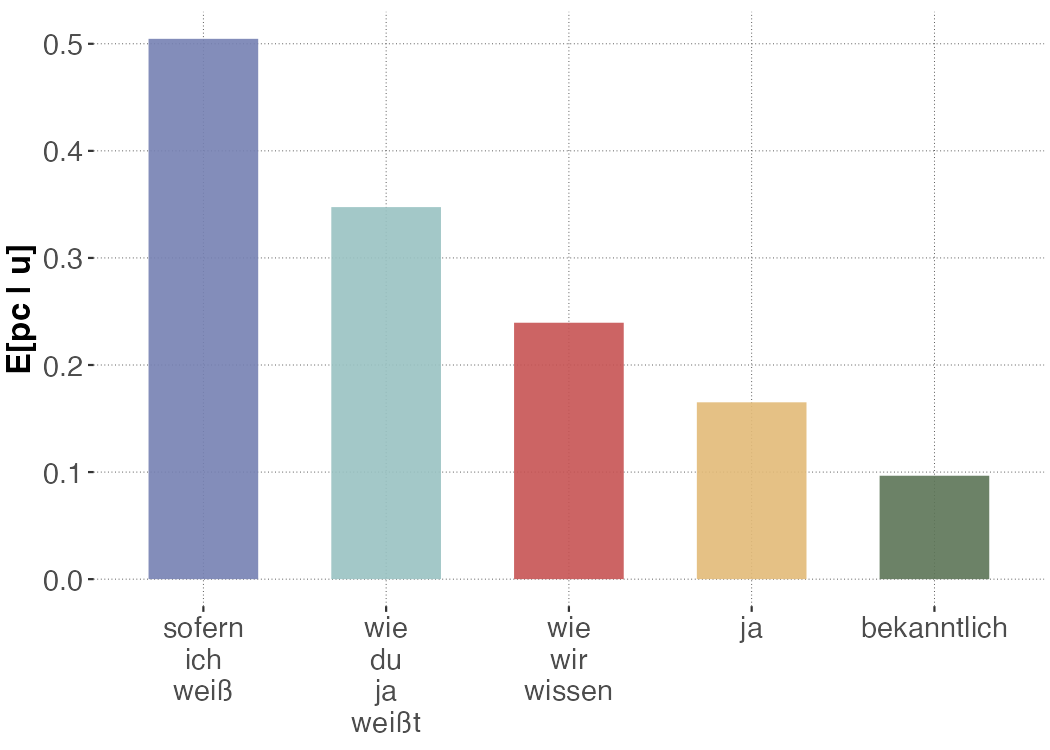
\includegraphics[width=\textwidth]{figures/pc_given_u.png}   % <-- replace with your filename
    \caption{Posterior expected perceived controversy $\mathbb{E}[pc \mid u]$ per marker.}
    \label{fig:pred_pc}
  \end{subfigure}
  \hfill
  \begin{subfigure}[b]{0.32\textwidth}
    \centering
    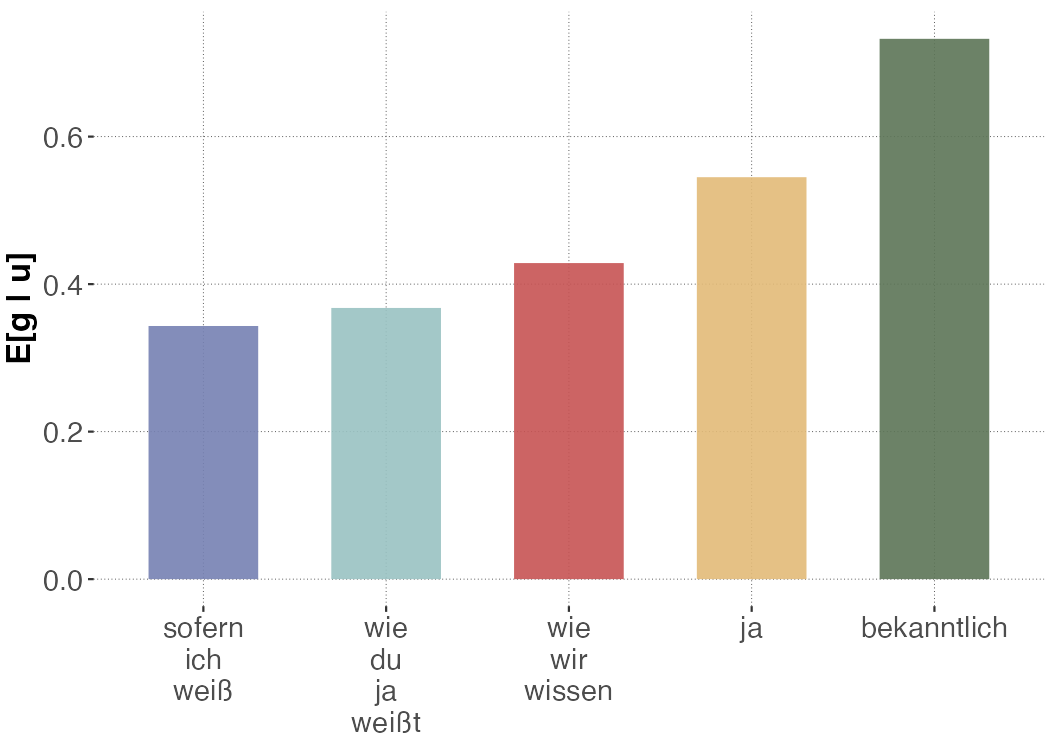
\includegraphics[width=\textwidth]{figures/g_given_u.png}    % <-- replace with your filename
    \caption{Posterior expected persuasive goal strength $\mathbb{E}[g \mid u]$ per marker.}
    \label{fig:pred_g}
  \end{subfigure}
  \hfill
  \begin{subfigure}[b]{0.32\textwidth}
    \centering
    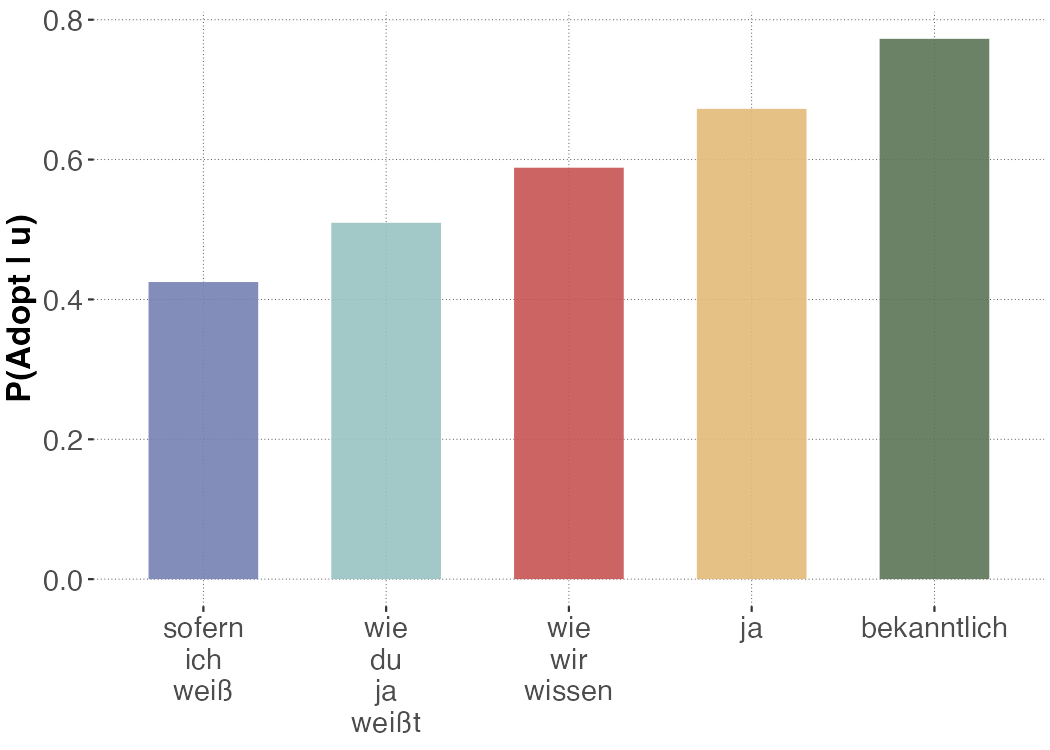
\includegraphics[width=\textwidth]{figures/adopt_given_u.png} % <-- replace with your filename
    \caption{Predicted action adoption probability $P(\mathrm{Adopt}(q) \mid u)$ per marker.}
    \label{fig:pred_adopt}
  \end{subfigure}
  \caption{}
  \label{fig:predictions}
\end{figure}

\begin{figure}[t]
  \centering
  \begin{subfigure}[b]{0.49\textwidth}
    \centering
    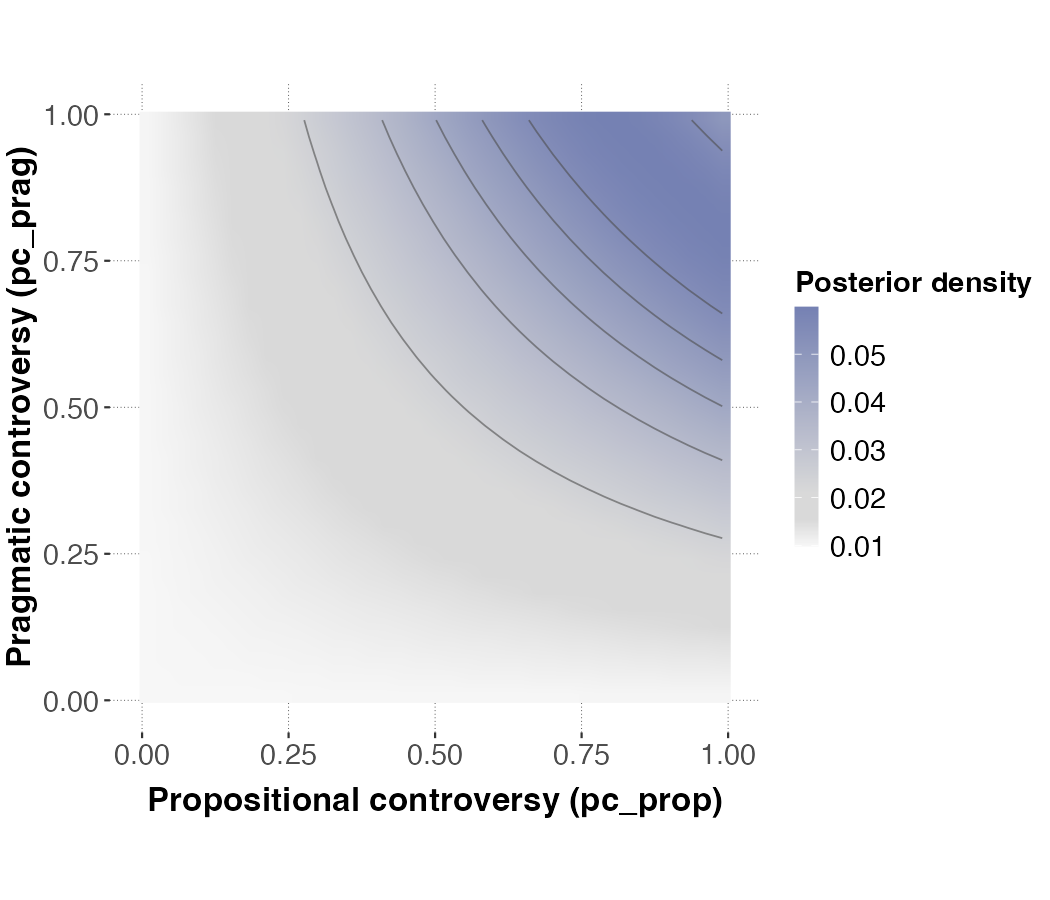
\includegraphics[width=\textwidth]{figures/int_pc_prop_pc_prag_weak.png}   % <-- replace with your filename
    \caption{TBD}
    \label{fig:pred_pc}
  \end{subfigure}
  \hfill
  \begin{subfigure}[b]{0.49\textwidth}
    \centering
    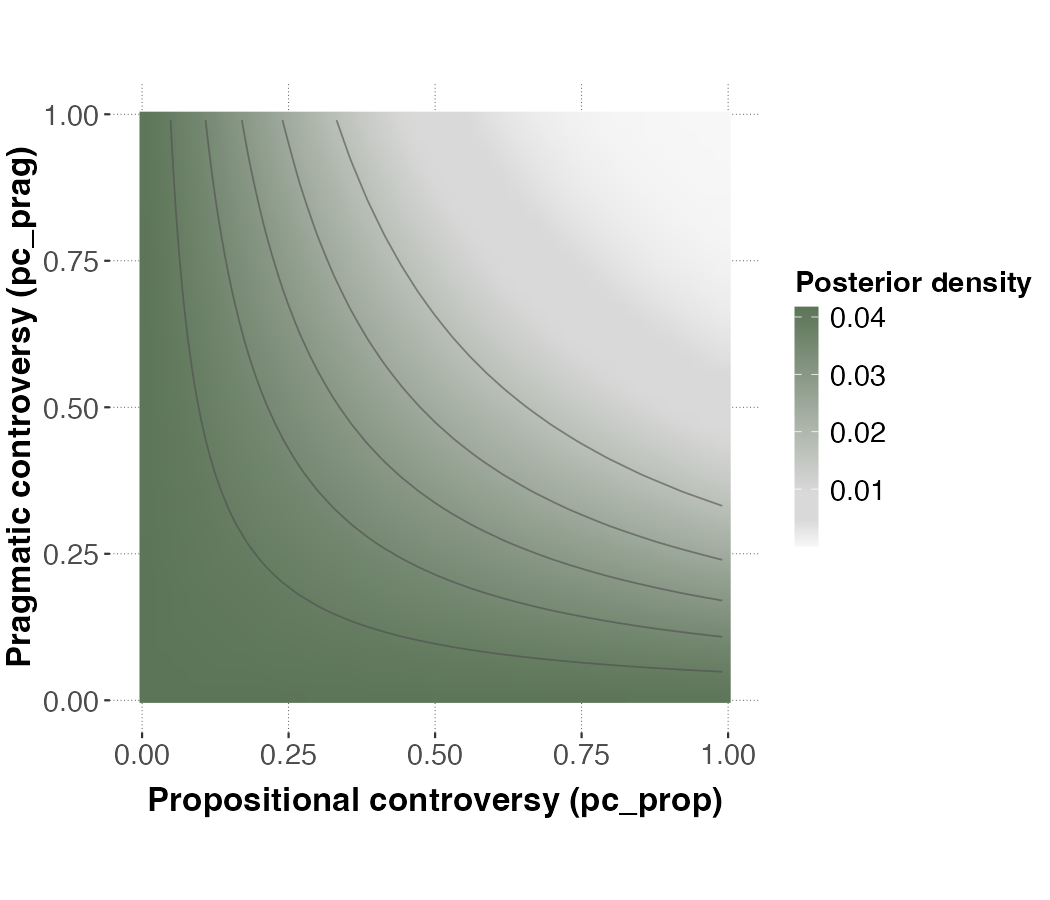
\includegraphics[width=\textwidth]{figures/int_pc_prop_pc_prag_strong.png}    % <-- replace with your filename
    \caption{TBD}
    \label{fig:pred_g}
  \end{subfigure}
  \caption{TBD}
  \label{fig:predictions}
\end{figure}

\begin{figure}[t]
  \centering
  \begin{subfigure}[b]{0.99\textwidth}
    \centering
    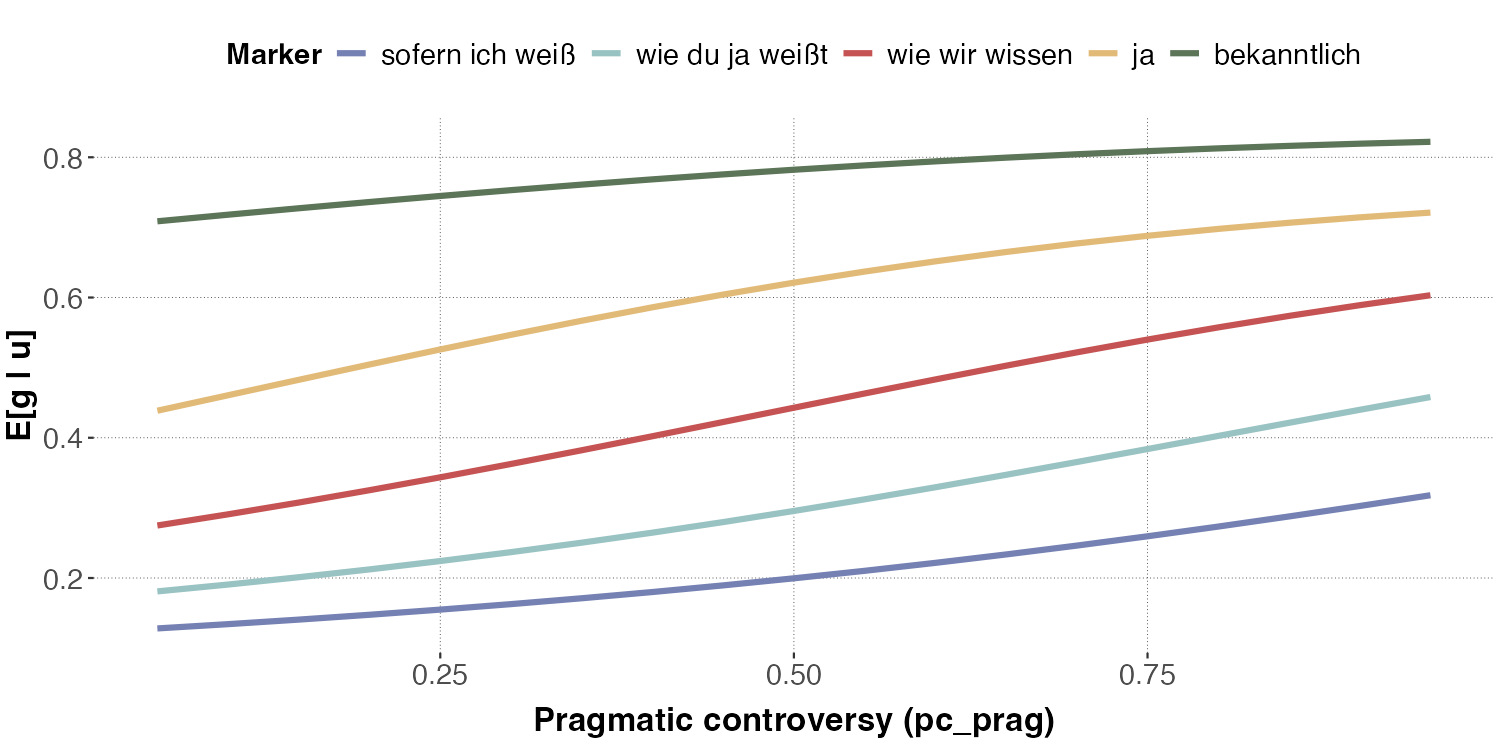
\includegraphics[width=\textwidth]{figures/int_pc_marker_g.png}   % <-- replace with your filename
    \caption{TBD}
    \label{fig:pred_pc}
  \end{subfigure}
    \caption{TBD}
  \label{fig:predictions}
\end{figure}

\begin{figure}[t]
  \centering
  \begin{subfigure}[b]{0.99\textwidth}
    \centering
    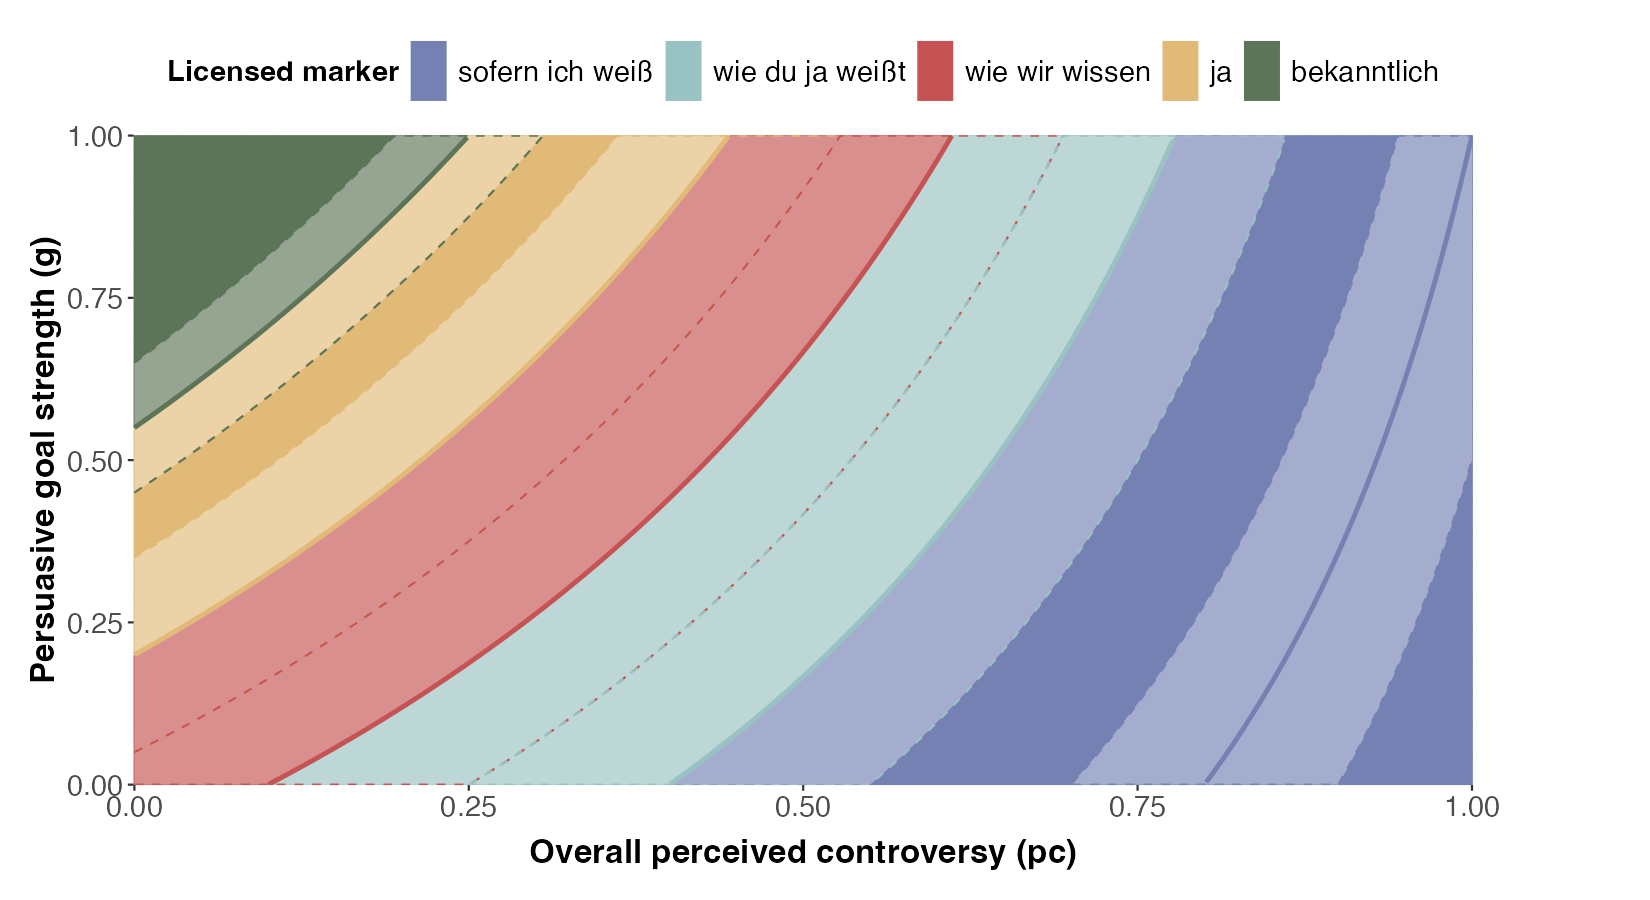
\includegraphics[width=\textwidth]{figures/util_landscape.png}   % <-- replace with your filename
    \caption{TBD}
    \label{fig:pred_pc}
  \end{subfigure}
    \caption{TBD}
  \label{fig:predictions}
\end{figure}


The comprehension model predicts systematic inferences about perceived controversy and speaker goal strength from the observed marker $u$, and downstream effects on action adoption.

\textbf{(1) Marker strength predicts lower overall perceived controversy.}
If markers lexicalize increasing thresholds
\[
\theta_{\text{sofern ich wei\ss}}
<
\theta_{\text{wie wir wissen}}
<
\theta_{\textit{ja}}
<
\theta_{\textit{bekanntlich}},
\]
then stronger markers license higher utility intervals and therefore support lower inferred overall controversy:
\[
\mathbb{E}[pc \mid u=\textit{bekanntlich}]
<
\mathbb{E}[pc \mid u=\textit{ja}]
<
\mathbb{E}[pc \mid u=\textit{wie wir wissen}]
<
\mathbb{E}[pc \mid u=\textit{sofern ich wei\ss}].
\]
In particular, stronger markers bias the listener towards interpretations in which $p$ is sufficiently settled in the relevant community.

\textbf{(2) Marker strength predicts higher inferred persuasive goal strength.}
Because stronger markers are licensed only when utility is high, and utility increases with $g$, observing a stronger marker shifts posterior mass toward higher $g$:
\[
\mathbb{E}[g \mid u=\textit{bekanntlich}]
>
\mathbb{E}[g \mid u=\textit{ja}]
>
\mathbb{E}[g \mid u=\textit{wie wir wissen}]
>
\mathbb{E}[g \mid u=\textit{sofern ich wei\ss}].
\]
Thus, consensus markers trigger theory-of-mind inferences about the speaker's intention to push the addressee toward adopting $q$.

\textbf{(3) Decomposition: propositional vs.\ pragmatic controversy.}
Since overall controversy is computed by
\[
pc = PC(pc_{\text{prop}},pc_{\text{prag}})=pc_{\text{prop}}\cdot pc_{\text{prag}},
\]
the model predicts a characteristic compensation pattern: high propositional controversy can be ``rescued'' by low pragmatic controversy (high community alignment), yielding low overall $pc$. Concretely, holding $pc_{\text{prop}}$ fixed, stronger markers push inferences toward lower $pc_{\text{prag}}$ (greater presumed alignment), whereas holding $pc_{\text{prag}}$ fixed, stronger markers push inferences toward lower $pc_{\text{prop}}$ (greater plausibility). This yields the prediction that the same marker can be licensed either by factual plausibility or by strong community alignment, and that listeners will trade off these sources of support in interpreting $u$.

\textbf{(4) Interaction between marker strength and controversy in inferred goal strength.}
Because the utility includes an interaction term $-(pc\cdot g)$, the effect of controversy on inferred goal strength is super-additive: under higher inferred $pc$, observing a strong marker forces a stronger increase in inferred $g$ in order to place the utterance within the marker's licensed utility interval. Thus, the model predicts the largest shifts in $\mathbb{E}[g \mid u]$ for strong markers in contexts where $p$ is (or would ordinarily be) controversial.

\textbf{(5) Downstream predictions for action adoption.}
Since adoption increases with $g$ and decreases with $pc$,
\[
P(\mathrm{Adopt}(q)\mid u)
\]
is predicted to be highest for strong markers when overall controversy is low, and reduced when overall controversy is high. Moreover, because marker strength jointly affects inferred $pc$ and $g$, the model predicts (i) higher adoption for stronger markers in low-controversy contexts, and (ii) a characteristic dissociation under high controversy: strong markers may still increase perceived persuasive pressure (higher $g$) even when willingness to act remains limited by high $pc$.

\section*{Experiments}

We test the comprehension--production connection implied by the model: (i) listeners infer perceived controversy and speaker goal strength from a consensus marker and use these in downstream action decisions; (ii) speakers choose markers as a function of inferred controversy and persuasive goal strength.

\subsection{General materials and factors}

\paragraph{Markers.}
The utterance $u$ contains one of five consensus markers (German):
\[
u \in \{\textit{sofern ich weiß},\ \textit{wie du ja weißt},\ \textit{wie wir wissen},\ \textit{ja},\ \textit{bekanntlich}\},
\]
assumed to lexicalize increasing thresholds $\theta_u$.

\paragraph{Proposition and action.}
Each item consists of a proposition $p$ (an informational claim) and a proposed action $q$ (a concrete recommendation). The target sentence frame is:
\[
\text{MARKER}(p)\ \ \Rightarrow\ \ \text{therefore adopt } q.
\]
Example (schematic):
\begin{quote}
\small
\textit{Bekanntlich} $p$ (``the new exam format yields more failing grades''). Therefore, $q$ (``we should postpone the exam reform'').
\end{quote}

\paragraph{Manipulating controversy.}
We orthogonally manipulate two sources of perceived controversy:

\begin{itemize}
\item \textbf{Propositional controversy} ($pc_{\text{prop}}$): plausibility/compatibility with world knowledge and evidence strength (e.g.\ strong vs.\ weak evidence; plausible vs.\ surprising claim).
\item \textbf{Pragmatic controversy} ($pc_{\text{prag}}$): expected disagreement / common-ground alignment in a specified community (e.g.\ shared expert consensus vs.\ polarized community).
\end{itemize}

\noindent Each item is paired with short contextual information implementing a $2 \times 2$ manipulation:
\[
pc_{\text{prop}} \in \{\text{low},\text{high}\}
\quad\times\quad
pc_{\text{prag}} \in \{\text{low},\text{high}\}.
\]
This directly targets the model decomposition $pc = PC(pc_{\text{prop}},pc_{\text{prag}})=pc_{\text{prop}}\cdot pc_{\text{prag}}$.

\paragraph{Pretests (recommended).}
We pretest contexts to validate that the manipulations selectively affect (i) plausibility/evidence ($pc_{\text{prop}}$) and (ii) expected disagreement/community alignment ($pc_{\text{prag}}$), using separate rating questions (see below).

% ==========================================================
\subsection{Experiment 1: Comprehension (inference + adoption)}

\paragraph{Goal.}
Test the listener-side predictions:
(i) marker strength drives inferences about $pc$ and $g$;
(ii) decomposition trade-off between $pc_{\text{prop}}$ and $pc_{\text{prag}}$;
(iii) downstream effects on $\Pr(\mathrm{Adopt}(q)\mid u)$.

\paragraph{Design.}
A mixed factorial design:
\begin{itemize}
\item \textbf{Within-item:} marker $u$ (4 levels).
\item \textbf{Within-item:} contextual manipulations $pc_{\text{prop}}$ (2) and $pc_{\text{prag}}$ (2).
\item \textbf{Random factors:} participant and item (crossed).
\end{itemize}
We use a Latin-square scheme so each participant sees each \emph{item} in exactly one marker condition (to avoid direct within-item comparisons of markers), while still seeing all factor levels across items.

\paragraph{Materials.}
Each trial shows:
\begin{enumerate}
\item a short vignette specifying an epistemic community $C$ (e.g.\ ``students in your department'', ``medical experts'', ``local residents''),
\item two context sentences implementing $pc_{\text{prop}}$ and $pc_{\text{prag}}$ (evidence strength vs.\ community alignment),
\item the target message: marker-applied claim $p$ followed by recommended action $q$.
\end{enumerate}

\paragraph{Procedure.}
For each trial, participants read the vignette and target message, then answer:

\begin{enumerate}
\item \textbf{Adoption decision (primary DV).}
\[
\text{Would you adopt } q?\ \ (\text{yes/no}) \quad\text{or}\quad \text{slider }[0,100].
\]
\item \textbf{Posterior proxies (inference DVs).}
\begin{itemize}
\item perceived overall controversy:
\[
\widehat{pc} \ \text{(``How controversial is $p$ in community $C$?'')} \in [0,100]
\]
\item perceived speaker goal strength:
\[
\widehat{g}\ \text{(``How strongly is the speaker trying to persuade you to do $q$?'')} \in [0,100]
\]
\item decomposition checks (optional but strongly recommended):
\[
\widehat{pc}_{\text{prop}}:\ \text{``How plausible is $p$ given the evidence?''}
\]
\[
\widehat{pc}_{\text{prag}}:\ \text{``How much disagreement would there be about $p$ in $C$?''}
\]
\end{itemize}
\item \textbf{Attention/understanding checks} (item-specific multiple-choice).
\end{enumerate}

\paragraph{Qualitative predictions.}
The model predicts:

\begin{enumerate}
\item \textbf{Marker strength $\rightarrow$ lower inferred controversy.}
Holding context fixed,
\[
\mathbb{E}[\widehat{pc}\mid u=\textit{bekanntlich}]
<
\mathbb{E}[\widehat{pc}\mid u=\textit{ja}]
<
\mathbb{E}[\widehat{pc}\mid u=\textit{wie wir wissen}]
<
\mathbb{E}[\widehat{pc}\mid u=\textit{sofern ich weiß}].
\]
\item \textbf{Marker strength $\rightarrow$ higher inferred persuasive goal strength.}
\[
\mathbb{E}[\widehat{g}\mid u=\textit{bekanntlich}]
>
\mathbb{E}[\widehat{g}\mid u=\textit{ja}]
>
\mathbb{E}[\widehat{g}\mid u=\textit{wie wir wissen}]
>
\mathbb{E}[\widehat{g}\mid u=\textit{sofern ich weiß}].
\]
\item \textbf{Compensation pattern (decomposition).}
Because $pc=pc_{\text{prop}}\cdot pc_{\text{prag}}$, a strong marker can be licensed either by
low $\widehat{pc}_{\text{prop}}$ (high plausibility) or low $\widehat{pc}_{\text{prag}}$ (high alignment).
Thus, effects of $u$ should partially manifest as shifts in both components.
\item \textbf{Downstream adoption.}
Adoption increases with $\widehat{g}$ and decreases with $\widehat{pc}$:
\[
\Pr(\mathrm{Adopt}(q)\mid u)
\ \text{is higher for stronger markers in low-controversy contexts,}
\]
with a dissociation under high controversy: strong markers can increase $\widehat{g}$ while adoption remains suppressed by high $\widehat{pc}$.
\end{enumerate}

\paragraph{Planned analysis (confirmatory).}
We estimate hierarchical regression models with crossed random effects (participant, item).

\begin{itemize}
\item \textbf{Inference models:}
\[
\widehat{pc} \sim u * pc_{\text{prop}} * pc_{\text{prag}} + (1+u\mid \text{participant}) + (1+u\mid \text{item})
\]
\[
\widehat{g} \sim u * pc_{\text{prop}} * pc_{\text{prag}} + (1+u\mid \text{participant}) + (1+u\mid \text{item})
\]
\item \textbf{Adoption model:}
\[
\Pr(\mathrm{Adopt}(q)) \sim u * pc_{\text{prop}} * pc_{\text{prag}} + (1+u\mid \text{participant}) + (1+u\mid \text{item})
\]
and (mediation-style) checks that $\widehat{pc}$ and $\widehat{g}$ statistically account for the marker effect:
\[
\Pr(\mathrm{Adopt}(q)) \sim u + \widehat{pc} + \widehat{g} + (1\mid\text{participant}) + (1\mid\text{item}).
\]
\end{itemize}

% ==========================================================
\subsection{Experiment 2: Production (marker choice under goals and controversy)}

\paragraph{Goal.}
Test the speaker-side implications of the utility-threshold semantics: speakers select markers as a function of (i) persuasive goal strength $g$ and (ii) perceived controversy $pc$, with particular sensitivity to the interaction $pc \cdot g$.

\paragraph{Design.}
A production-choice task with manipulated communicative goals and context:

\begin{itemize}
\item \textbf{Goal strength} $g$ (2--3 levels; manipulated via incentives/instructions):
\[
g \in \{\text{low (inform)},\ \text{medium (recommend)},\ \text{high (persuade/pressure)}\}.
\]
\item \textbf{Contextual controversy:} the same $2\times 2$ manipulation of $pc_{\text{prop}}$ and $pc_{\text{prag}}$ as in Experiment~1.
\item \textbf{Outcome:} marker choice $u$ (4-way categorical), plus optional free-text realization.
\end{itemize}

\paragraph{Materials.}
Each trial provides:
\begin{enumerate}
\item the vignette (community $C$) and evidence/alignment information (implementing $pc_{\text{prop}}, pc_{\text{prag}}$),
\item the content to communicate: the proposition $p$ and the intended action recommendation $q$,
\item a role/goal instruction manipulating $g$.
\end{enumerate}

\paragraph{Goal manipulation (examples).}
\begin{itemize}
\item \textbf{Low $g$ (informative):} ``Your task is to neutrally inform the addressee about $p$. Do not try to influence their action.''
\item \textbf{High $g$ (persuasive):} ``Your task is to get the addressee to adopt $q$. You have limited time and need to be effective.''
\end{itemize}
Optionally, add an incentive-compatible bonus tied to the addressee's (simulated or real) adoption to operationalize $g$.

\paragraph{Procedure.}
On each trial, participants construct the message by selecting a marker from a drop-down menu:
\[
\text{[marker]} + p \quad\text{then}\quad \text{recommend } q.
\]
Optionally, participants can also edit the full sentence to allow naturalistic production, while the marker choice remains the main DV.

After producing the message, participants provide manipulation checks:
\[
\widehat{pc}_{\text{prop}},\ \widehat{pc}_{\text{prag}},\ \widehat{g}
\]
(brief slider questions to verify that the intended goal and context were perceived as such).

\paragraph{Predictions.}
Let marker strength correspond monotonically to $\theta_u$.

\begin{enumerate}
\item \textbf{Goal strength increases marker strength.}
Higher instructed $g$ yields a higher probability of selecting strong markers:
\[
\Pr(u=\textit{bekanntlich}\ \text{or}\ \textit{ja} \mid g=\text{high})
>
\Pr(u=\textit{bekanntlich}\ \text{or}\ \textit{ja} \mid g=\text{low}).
\]
\item \textbf{Controversy decreases marker strength.}
Higher $pc$ reduces the use of strong markers, due to the cost term in $U(p;pc,g)$.
\item \textbf{Interaction: controversy $\times$ goal.}
Because $U$ contains $-(pc\cdot g)$, the effect of $g$ on marker choice is attenuated when $pc$ is high:
strong markers are most favored when $g$ is high \emph{and} $pc$ is low; conversely, when $pc$ is high, even high $g$ yields more conservative markers.
\item \textbf{Decomposition trade-off.}
High $pc_{\text{prop}}$ can be compensated by low $pc_{\text{prag}}$ (and vice versa). Thus, strong markers should be more likely in mixed cases (high/low) than in high/high.
\end{enumerate}

\paragraph{Planned analysis.}
We model marker choice with an ordinal or multinomial mixed-effects model.

\begin{itemize}
\item \textbf{Ordinal approach:} map markers to an ordered scale by assumed $\theta_u$ and fit:
\[
u_{\text{strength}} \sim g * pc_{\text{prop}} * pc_{\text{prag}} + (1\mid \text{participant}) + (1\mid \text{item}).
\]
\item \textbf{Multinomial approach:} directly predict categorical $u$:
\[
\Pr(u=k) = \text{softmax}_k(\beta_{0k} + \beta_{gk} g + \beta_{pk} pc_{\text{prop}} + \beta_{rk} pc_{\text{prag}} + \cdots),
\]
with participant/item random intercepts (and slopes where identifiable).
\end{itemize}

\paragraph{Linking production and comprehension.}
A key cross-experiment test is whether the production pattern aligns with the comprehension-inferred thresholds:
the same ordering of marker strength that drives lower inferred $\widehat{pc}$ and higher inferred $\widehat{g}$ in Experiment~1
should also be selected more frequently when speakers face low controversy and higher persuasive goals in Experiment~2.

\paragraph{Optional extension: closing the loop.}
To directly validate the downstream decision component, we can run a \emph{yoked design}:
messages produced in Experiment~2 are shown to new participants in a comprehension/adoption task (Experiment~1),
testing whether naturally produced marker choices causally shift $\widehat{pc}$, $\widehat{g}$, and $\Pr(\mathrm{Adopt}(q))$ as predicted.

\printbibliography

\end{document}   
\begin{comment}

\newpage
\section{Abstract-V0.1}
\newpage
\textbf{\large From Controversy to Consensus: Modeling Community-Sensitive Common-Ground Management in German Discourse Markers}

Discourse particles such as \textit{ja} are ubiquitous in German, yet their formal modeling has proven challenging. Standard accounts converge on the idea that \textit{ja} signals that a proposition $p$ is, in some relevant sense, already settled. It has been described as marking $p$ as \textsc{known} \citep{thurmair1989modalpartikeln}, as indicating (speaker-assumed) common knowledge \citep{karagjosova2004meaning}, or as conveying that $p$ is uncontroversial (and possibly true) \citep{jacobs_semantics_1991,zimmermann2011discourse,waltereit2001modal}. 


While these notions differ in detail, they arguably target a shared core intuition: the speaker presents $p$ as not up for dispute in the current discourse. This intuition has been implemented in different ways — for instance, \yg{by stating that $\neg p$ is not part of the Common Ground (CG), or by analyzing the contribution as a presupposition that the speaker believes the addressee does not actively consider the possibility of $\neg p$, which means that neither $p$ nor $\neg p$ is under discussion.} as the absence of active consideration of $\neg p$ in the common ground (CG), or as a presupposition that the addressee is not currently attending to $p$. Moreover, \citet{doring2016modal} argues that \textit{ja} can be used strategically to support broader communicative goals, a function already foreshadowed in \citet{thurmair1989modalpartikeln}. \yg{These goals can be understood as the facilitation of discourse continuation: by presenting $p$ as uncontroversial, \textit{ja} increases discourse stability and promotes smooth progression within the evolving discourse structure.} Recent experimental work by \citet{seemann2025} further suggests that the use of \textit{ja} is closely tied to causal reasoning contexts.

However, several empirical and conceptual gaps remain.

First, the notion of \emph{uncontroversiality} is rarely defined with precision. In particular, previous accounts do not capture the fact that controversy is community-relative: a proposition may be uncontroversial within one epistemic community but controversial in another (e.g., conspiracy-theoretic vs.\ scientific communities). Furthermore, some propositions are inherently controversial due to violations of world knowledge or linguistic conventions. Consider the examples in (\ref{ex:impfung-neutral})–(\ref{ex:impfung-convince}).

\begin{exe}
    \ex Impfungen sind \#ja sicher und wirksam. \label{ex:impfung-neutral}
    \ex (Speaking to medical scientists) Impfungen sind ja sicher und wirksam. \label{ex:impfung-positvecommunity}
    \ex Impfungen sind ja sicher und wirksam. Alle sollen sich impfen lassen! \label{ex:impfung-convince}
\end{exe}

%Another example:
%\begin{exe}
   % \ex Vegane Ernährung ist \#ja gesund. \label{ex:meat-eater}
   % \ex (Speaking to vegan) Vegane Ernährung ist ja gesund. \label{ex:vegan-community}
   % \ex Vegane Ernährung ist ja gesund. Man sollte Fleisch aufgeben. \label{ex: vegan-convince}
%\end{exe}

In a general public setting, the proposition that vaccines are safe and effective may be perceived as controversial, which degrades the felicity of consensus markers such as \textit{ja} (\ref{ex:impfung-neutral}). In contrast, within a community of medical scientists, the same proposition is considerably less controversial, licensing \textit{ja} (\ref{ex:impfung-positvecommunity}). Finally, in persuasive contexts, \textit{ja} may be used strategically to pave the ground for a subsequent directive or argument (\ref{ex:impfung-convince}), even when controversy is present.

Second, manipulative or strategic uses of \textit{ja} suggest that communicative goals can partially override baseline controversy assessments. That is, speakers may present $p$ as settled precisely in order to shape the subsequent discourse.

We build on two strands of prior work. First, following \citet{repp2013common}, we treat \textit{ja} and related expressions as CG-management markers: rather than contributing to propositional content \citep{grosz2021discourse}, they signal the common-ground status of $p$, in particular that $p$ is treated as already part of the CG and retrievable from prior discourse. \yg{Upon retrieval, \textit{ja} reactivates the proposition, making it salient within the current conversational context.This characterization of \textit{ja} is modeled as a use-conditional constraint linked to communicative goals \citep{gutzmann2015use}} This retrieval component can be modeled as a use-conditional constraint tied to communicative goals \citep{gutzmann2015use}. 

Second, building on \citet{seemann2025}, we take seriously the observation that \textit{ja} is frequently embedded in causal reasoning contexts, where it helps establish premises for subsequent argumentative moves \citep{doring2016modal}. This suggests that any formal account must integrate (i) a model of common ground and (ii) a model of controversy that interacts with goal-directed communication.

This study focuses on a class of German discourse markers — \textit{ja}, \textit{wie wir wissen} (‘as we know’), and \textit{bekanntlich} (‘as is well known’) — which we group under the label \emph{consensus markers}. We propose to the meaning of such markers consisting of two sources of utlities: literal meaning (used to expressed) and uncontroversiality (property of p itself). uncontroversiality is defined also via two components: A distinction between \emph{propositional} and \emph{pragmatic} controversy, both evaluated relative to a community. Their interaction yields a measure of perceived controversy.

\begin{enumerate}
    \item 
    \item A utility-based component reflecting communicative goals in a causal-reasoning setting \citep{seemann2025}, incorporating (i) beliefs about the common ground (what the listener is taken to know) and (ii) the speaker’s private belief strength.
\end{enumerate}

By integrating these components, we posit that each consensus marker lexicalizes a threshold over a weighted utility function: the stronger the marker, the stronger the required signal that $p$ is treated as settled, formally we have:

\begin{equation}
\begin{aligned}
\llbracket \text{CG-MARKER}\rrbracket(g,c,w) &= \lambda p: util(u) > \theta \\
&\text{a. } [\text{PS}_S(p, c) \geq \alpha_{\text{marker}}] \quad \text{UTILITY OF COMMUNICATION} \\
&\text{b. } [\text{PC}(G_{\text{marker}}, p, w) \leq \theta_{\text{marker}}] \quad \text{PERCEIVED-CONTROVERSY} \\
&\text{c. } [\text{UTILITY}(\text{PS}_S(p, c), \text{PC}(G_{\text{marker}}, p, w)) > \beta_{\text{marker}}] \quad \text{FELICITY}
\end{aligned}
\label{eq:cg-marker-refined}
\end{equation}



\newpage


%Scholars diverge in how they conceptualize uncontroversiality. Thurmair (1989) characterizes it in terms of the feature KNOWN, namely that the proposition is already known to the addressee and thus forms part of the Common Ground. Jacobs (1991), by contrast, treats uncontroversiality as a felicity condition on the illocutionary operator ASSERT: the speaker assumes that the addressee believes that p holds, or at least does not believe p to be false nor consider its falsity a live possibility in the given context. Adopting a speech-act-theoretical perspective, Waltetreit (2001) likewise links uncontroversiality to discourse conditions, but broadens it to include not only prior knowledge but also the availability of sufficient evidence for p.




    



where
$\text{PS}_S(p, c) := \text{BEL}_S(p) \times \text{CG-ESTABLISHMENT}_S(p, c)$
and
$\text{PC}(G, p, w) := I(p) \times (1 - \frac{|\{a \in G : \text{Acc}(a,p)(w) = 1\}|}{|G|})$
\subsection*{Perceived Controversy: A Two-Component Model}

Perceived controversy comprises two components: \textbf{propositional (inherent) controversy} and \textbf{pragmatic controversy}. The former is an inherent property of the proposition itself. Let $I(p)$ be the inherent controversy function:

\begin{equation}
I : \langle s,t\rangle \to [0,1]
\label{eq:inherent-controversy}
\end{equation}

where higher values indicate greater inherent controversy. We will use a norming study to elicit human priors to operationalize $I(p)$.

\paragraph{Example (inherent controversy).}
Consider the propositions \textit{``Zitronen sind sauer''} vs.\ \textit{``Bonbons sind sauer''}. The former has low inherent controversy ($I(p) \approx 0.1$) insofar as it expresses established background knowledge grounded in stable sensory experience and lexical categorization. By contrast, the latter exhibits higher inherent controversy ($I(p) \approx 0.5$) because candies vary considerably in flavor profile, and whether they count as sour depends on subtype, individual taste perception, and contextual standards.

\paragraph{Pragmatic controversy.}
Pragmatic controversy is a property of the common ground: it depends on how firmly a proposition is (taken to be) established as shared within a relevant community $G$.\footnote{The choice of $G$ can be tied to cultural communities and their associated shared bases, yielding communal common ground, as opposed to personal common ground based on direct interaction.}%
Different communities exhibit different degrees of consensus, which affects how controversial $p$ is perceived to be in that community.

\subsection*{Formal Framework: Acceptance, Coverage, and Pragmatic Controversy}

Let $A$ be the set of agents. Acceptance is defined as:

\begin{equation}
\text{Acc} : A \times \langle s,t\rangle \to \langle s,t\rangle
\label{eq:acceptance}
\end{equation}

\begin{equation}
\text{Acc}(a,p)(w) = 1 \text{ iff } a \text{ accepts } p \text{ in } w
\label{eq:acceptance-condition}
\end{equation}

For any group $G \subseteq A$, define the \emph{acceptance rate} (coverage) of $p$ in $G$:

\begin{equation}
\text{Cov}(G,p,w) \ :=\ \frac{|\{a \in G : \text{Acc}(a,p)(w)=1\}|}{|G|}
\label{eq:coverage}
\end{equation}

This yields a thresholded notion of (sufficient) mutual group acceptance:

\begin{equation}
\text{MG}_{\rho}(G,p) \ :=\ \lambda w.\ \text{Cov}(G,p,w)\ \ge\ \rho
\label{eq:mutual-group-acceptance-threshold}
\end{equation}

Pragmatic controversy is then defined as inherent controversy modulated by community coverage:

\begin{equation}
\text{PC}(G,p,w)\ :=\ I(p)\cdot\bigl(1-\text{Cov}(G,p,w)\bigr)
\label{eq:pragmatic-controversy}
\end{equation}

\paragraph{Example (pragmatic controversy varies with $G$).}
Consider the proposition \textit{``Vaccines are safe and effective for preventing infectious diseases''}. Even if $I(p)$ is held fixed, pragmatic controversy varies across communities:
\begin{align}
\textbf{Medical professional community } G_{\text{med}}: \quad \text{PC}(G_{\text{med}},p,w)
&= I(p)\cdot(1-0.95)\ \approx\ \text{low} \\
\textbf{Vaccine-hesitant community } G_{\text{hesit}}: \quad \text{PC}(G_{\text{hesit}},p,w)
&= I(p)\cdot(1-0.25)\ \approx\ \text{high}
\end{align}

\subsection*{Private Strength vs.\ Perceived Controversy in CG-Markers}

CG-markers are sensitive both to (i) a \textbf{private strength} component and (ii) a \textbf{community-based perceived-controversy} component. The private component is intended to track not only whether the speaker believes $p$, but also the speaker's assessment of how established (and retrievable) $p$ is in the common ground, including salience-related factors. This aligns with analyses on which certain particles (e.g.\ \textit{ja}) manage common ground and (re-)activate non-salient shared information, and on which \textit{ja} contributes an uncontroversiality-related component.

\paragraph{Private strength.}
\begin{equation}
\text{PS}_S(p,c)\ :=\ \text{BEL}_S(p)\ \times\ \text{CG-ESTABLISHMENT}_S(p,c)
\label{eq:private-strength}
\end{equation}

\paragraph{Lexical meaning schema.}
\begin{equation}
\begin{aligned}
\llbracket \text{CG-MARKER}\rrbracket^{g,c,w}
&= \lambda p_{\langle s,t\rangle}:\ 
\text{PS}_S(p,c)\ \ge\ \alpha_{\text{marker}} \\
&\ \ \ \ \ \ \ \ \ \ \ \ \ \ \ \ \ \ \ \ \land\ \text{PC}(G_{\text{marker}},p,w)\ \le\ \theta_{\text{marker}} \\
&\ \ \ \ \ \ \ \ \ \ \ \ \ \ \ \ \ \ \ \ \land\ \text{U}\bigl(\text{PS}_S(p,c),\text{PC}(G_{\text{marker}},p,w)\bigr)\ >\ \beta_{\text{marker}}.\ p
\end{aligned}
\label{eq:cg-marker-refined}
\end{equation}

Here, $\alpha_{\text{marker}}$ and $\theta_{\text{marker}}$ are lexical thresholds, and $\text{U}$ encodes the idea that felicity depends on a \emph{trade-off} between private strength and perceived controversy (rather than requiring either component to dominate categorically). One simple implementation is:

\begin{equation}
\text{U}(\text{PS},\text{PC})\ :=\ \omega_{\text{PS}}\cdot \text{PS}\ -\ \omega_{\text{PC}}\cdot \text{PC}
\label{eq:utility}
\end{equation}

\paragraph{Private belief can ``overwrite'' perceived controversy (trade-off).}
Because felicity is mediated by $\text{U}$, a speaker with very high private strength may still use a strong CG-marker even when $\text{PC}(G_{\text{marker}},p,w)$ is comparatively high (e.g.\ as a strengthening or potentially manipulative move in argumentation, i.e.\ presenting $p$ as settled for conversational purposes). This is compatible with approaches that treat certain items as CG-managing operators, i.e.\ operators that constrain how $p$ is to be treated relative to the CG (commitment, expectedness, retrieval), rather than merely contributing truth-conditional content.

Example: In a public debate with an audience $G_{\text{pub}}$ that is divided on $p$, a speaker with high $\text{PS}_S(p,c)$ may say: \textit{``Impfungen sind bekanntlich sicher und wirksam.''} The marker frames $p$ as broadly established despite audience disagreement, aiming to push $p$ toward a ``settled'' CG-status.

\subsection*{Scalar Community Structure for CG-Strengthening Markers}

Each marker is associated with (i) a \emph{community parameter} $G_{\text{marker}}$ and (ii) lexical thresholds $(\alpha_{\text{marker}},\theta_{\text{marker}})$.
Intuitively, stronger markers require broader community consensus (lower tolerated $\theta$) and/or a larger relevant community $G$ (communal common ground), whereas weaker markers can be licensed with smaller $G$ and/or higher tolerated $\theta$ (personal common ground).

A schematic lexicon fragment:

\begin{equation}
\begin{array}{lccc}
\text{Marker} & G_{\text{marker}} & \alpha_{\text{marker}} & \theta_{\text{marker}} \\
\hline
\textit{bekanntlich} & \text{Comm}(c) & 0.9 & 0.1 \\
\textit{wie wir wissen} & G_{\text{in-group}}(c) & 0.7 & 0.3 \\
\textit{wie du ja wei\ss t} & \{S,H\} & 0.6 & 0.4 \\
\textit{ja} & \{S,H\} & 0.5 & 0.5 \\
\textit{sofern ich wei\ss} & \{S\} & 0.3 & 0.7 \\
\end{array}
\label{eq:marker-lexicon}
\end{equation}

The community parameters can be ordered by inclusion (keeping in mind that \textit{wie du ja wei\ss t} and \textit{ja} may share the same dyadic $G$ but differ in thresholds and/or in the private-strength requirement):

\begin{equation}
\{S\}\ \subset\ \{S,H\}\ \subset\ G_{\text{in-group}}(c)\ \subset\ \text{Comm}(c)
\label{eq:community-inclusion}
\end{equation}

Finally, for convenience (equivalent to \eqref{eq:pragmatic-controversy}), the marker-indexed pragmatic controversy can be written as:

\begin{equation}
\text{PC}(G_{\text{marker}},p,w)\ =\ I(p)\cdot\left(1-\frac{|\{a\in G_{\text{marker}}:\text{Acc}(a,p)(w)=1\}|}{|G_{\text{marker}}|}\right)
\label{eq:pc-marker}
\end{equation}

    
\end{comment}


%\begin{exe}
   % \ex Xelieherb ist ja/wie wir wissen/bekanntlich assoziiert mit Ralocrop. Wir sollen mehr ralocrop anbauen. (High controversial + High private belief)
   % \ex Xelieherb ist ja/wie wir wissen assoziiert mit Ralocrop. Sollen wir mehr ralocrop anbauen? (ja/wie wir wissen/\#bekanntlich + low private belief) 
   % \ex Rauchen ist ja/wie wir wissen/bekanntlich wissen assoziiert mit Krebs. Wir sollen aufhören zu rauchen. (low controversial + high private belief)
  %  \ex Rauchen ist ja/wie wir wissen/\#bekanntlich wissen assoziiert mit Krebs. Sollen wir aufhören zu rauchen? (low controversial + low private belief)
%\end{exe}
\end{comment}

\begin{comment}
\textbf{The Computational Model (RSA)}  

We formalize the pragmatics of CG management markers within the Rational Speech Act (RSA) framework. Standard RSA models define a utility function $U$ based on informativity (reduction of uncertainty). We extend this to include a \textit{social management} component.  

We operationalize the qualitative notion of **uncontroversiality** as the prior probability of a proposition, $P(w)$, within the shared belief space (the assumed Common Ground).   
\begin{itemize}  
    \item **Controversy** is formalized as $1 - P_{CG}(p)$. A proposition is ``uncontroversial'' if $P_{CG}(p) \approx 1$.  
    \item **Private Belief** is formalized as the speaker's internal probability $P_{S}(p)$.  
\end{itemize}  

We hypothesize that particles like \textit{ja} and \textit{bekanntlich} act as presuppositional filters or costly signals that are licensed only when $P_{CG}(p)$ exceeds a specific threshold $\theta$. In our RSA model, the speaker $S$ chooses an utterance $u$ (from options: \textit{ja}, \textit{wie wir wissen}, \textit{bekanntlich}, $\emptyset$) to maximize utility, where the utility of using a particle is penalized if the divergence between the assumed CG and the particle's requirement is high.  

\textbf{Experimental Design}  

To validate this formalization, we conduct two related studies, where the first establishes the empirical inputs for the second. 

\textbf{Study 1: Normative Elicitation of Controversy} 

To derive grounded inputs for our production model, we first conducted a normative study. We selected a set of 40 propositions ranging from scientific truisms (e.g., ``The earth revolves around the sun'') to widely debated topics and clearly false statements. 
The 40 propositions were primarily divided into two broad categories: world knowledge (Weltwissen) and linguistic knowledge (Sprachwissen). The latter comprises propositions whose relevant property is lexically encoded. We predict that propositions belonging to linguistic knowledge will cluster at the extremes of inherent controversy. Specifically, they are expected to occur either in cases of very low controversy (I(p) = 0), such as “Lemons are sour”, where the property is prototypically and lexically associated with the subject, or in cases of maximal controversy (I(p) = 1), such as “Bus rides are sour”, which violates lexical-semantic conventions.

In contrast, the category of world knowledge is expected to display a more fine-grained, scalar distribution of uncontroversiality. We distinguish several subtypes. First, trivial knowledge, including everyday norms (e.g., “One stops at red lights”), scientific truisms (e.g., “The earth is round.”), and widely known factual information (e.g., “Margaret Thatcher was the first female Prime Minister of the UK” or “The capital of Germany is Berlin.”). Second, traditionally transmitted beliefs, encompassing socially or culturally inherited assumptions (e.g., “Being a doctor is a respectable profession”). Third, proverbs (e.g., “Time is money.”). Fourth, shared conceptualizations of particular objects (e.g., “Apples are sour”). Finally, we include widely debated societal issues, such as refugee policy or the health effects of vegan diets.

Crucially, because shared knowledge is evaluated relative to a community, the community itself constitutes a central factor in determining whether a proposition is perceived as controversial. To capture this community-relativity, we embedded the above subtypes in explicitly specified community contexts. In particular, we targeted distinct epistemic communities — for example, German vegans versus German meat-eaters — who may systematically differ in their assessments of the same proposition. We therefore expect that identical propositions will receive different controversy ratings depending on the community context against which they are evaluated.

Participants were recruited from two distinct communities differing in their ideological orientation (e.g., German vegans and German meat-eaters), with N = 30 participants per group. Each group rated the same set of propositions on a Likert scale with respect to their perceived level of general societal agreement within their respective community. These ratings provide the numerical values for the **Controversy** variable (the prior $P_{CG}(p)$) used in Study 2.  

\textbf{Study 2: Production Experiment}  

This study investigates how German consensus markers (\textit{ja, wie wir wissen, bekanntlich}) are licensed in causal reasoning contexts as a function of perceived controversy and private belief strength. Building on a community-indexed model of controversy derived in Study 1, we conduct a $2 \times 2$ within-subject design production experiment manipulating:

\begin{enumerate}  
    \item \textbf{Community-relative controversy (High vs. Low):} Selected based on Study 1 scores (e.g., vegan vs. meat-eater communities evaluating the proposition \textbf{Eine vegane Ernährung ist mit gesundheitlichen Vorteilen assoziiert}).  
    \item \textbf{Strength of Private Belief (High vs. Low):} Manipulated via the context provided to the participant (e.g., ``You have read a definitive report...'' vs. ``You vaguely remember hearing...'').  
\end{enumerate}  

\textbf{Task:} Participants read a short context vignette establishing the strength of their private belief regarding a proposition with a known controversy score. They are then asked to complete a sentence by selecting the most natural expression from a drop-down menu.  
\\

We predict that marker choice reflects a weighted interaction between perceived controversy and communicative utility. In low-controversy contexts with strong private belief, stronger consensus markers (e.g., \textit{bekanntlich, wie wir wissen}) are expected to be preferred. In low-belief contexts, weaker marking or null assertion should dominate. Crucially, in high-controversy contexts, strong private belief may strategically license \textit{ja}, reflecting an override of baseline controversy in service of persuasive goals. These patterns provide empirical support for a threshold-based computational model in which consensus markers lexicalize graded signals of “settledness” over a utility-weighted representation of common ground and speaker conviction.

%\textbf{Options:}  
%\begin{itemize}  
    %\item \textit{Das ist ja...} (It is \textit{ja}...)  
    %\item \textit{Wie wir wissen, ist das...} (As we know, it is...)  
    %\item \textit{Bekanntlich ist das...} (As is well known, it is...)  
   % \item \textit{Das ist...} (Null marking / simple assertion)  
%\end{itemize}  

\textbf{Example}
\textbf{Target proposition}

\textit{Eine vegane Ernährung ist mit gesundheitlichen Vorteilen assoziiert.}

Assumed results from study 1:
\begin{itemize}
    \item In the German vegan community --> Low Controversy
    \item In the German meat-eater community --> High Controversy
\end{itemize}

\textbf{Condition 1}

\textbf{Low Controversy (Vegan Community) + High Private Belief}

\textbf{Community vignette}

Stell dir vor, du schreibst in einem deutschen Vegan-Forum.

\textbf{Private belief manipulation}

Du hast gerade eine ausführliche Meta-Analyse einer anerkannten medizinischen Fachzeitschriften gelesen, die klare gesundheitliche Vorteile einer gut geplanten veganen Ernährung zeigt. Du bist vollkommen überzeugt.

\textbf{Taget}
Eine vegane Ernährung ist \underline{\hspace{1cm}} mit gesundheitlichen Vorteilen assoziiert. Wir sollten auf Fleisch verzichten.
\begin{itemize}
    \item bekanntlich
    \item wie wir wissen
    \item ja
    \item $\emptyset$ (Null marking )
\end{itemize}


\textbf{Condition 2}

\textbf{Low Controversy (Vegan Community) + Low Private Belief}

\textbf{Community vignette}

Stell dir vor, du schreibst in einem deutschen Vegan-Forum.

\textbf{Private belief manipulation}

Du hast davon schon öfter gehört, erinnerst dich aber nur vage an Details und bist dir nicht ganz sicher, wie eindeutig die Evidenz ist, dass eine vegane Ernährung gesundheitliche Vorteile zeigt.

\textbf{Taget}
Eine vegane Ernährung ist \underline{\hspace{1cm}} mit gesundheitlichen Vorteilen assoziiert. Sollten wir vielleicht versuchen, auf Fleisch zu verzichten?
\begin{itemize}
    \item bekanntlich
    \item wie wir wissen
    \item ja
    \item $\emptyset$ (Null marking )
\end{itemize}

\textbf{Condition 3}

\textbf{High Controversy (Meat-eater Community) + High Private Belief}

\textbf{Community vignette}

Stell dir vor, du schreibst in einem deutschen Grill- und Fleischliebhaber-Forum.

\textbf{Private belief manipulation}

Obwohl dieses Thema hier häufig skeptisch diskutiert wird, hast du gerade eine ausführliche Meta-Analyse einer anerkannten medizinischen Fachzeitschrift gelesen, die klare gesundheitliche Vorteile einer gut geplanten veganen Ernährung zeigt. Du bist vollkommen überzeugt.

\textbf{Taget}
Eine vegane Ernährung ist \underline{\hspace{1cm}} mit gesundheitlichen Vorteilen assoziiert. Wir sollten auf Fleisch verzichten.
\begin{itemize}
    \item bekanntlich
    \item wie wir wissen
    \item ja
    \item $\emptyset$ (Null marking )
\end{itemize}

\textbf{Condition 4}

\textbf{High Controversy (Meat-eater Community) + Low Private Belief}

\textbf{Community vignette}

Stell dir vor, du schreibst in einem deutschen Grill- und Fleischliebhaber-Forum.

\textbf{Private belief manipulation}

In dieser Community wird das Thema häufig kontrovers diskutiert, ob eine vegane Ernährung gesundheitliche Vorteile zeigt. Du hast davon schon gehört, bist dir aber nicht sicher, wie überzeugend die Evidenz ist.

\textbf{Taget}
Eine vegane Ernährung ist \underline{\hspace{1cm}} mit gesundheitlichen Vorteilen assoziiert. Sollten wir vielleicht versuchen, auf Fleisch zu verzichten?
\begin{itemize}
    \item bekanntlich
    \item wie wir wissen
    \item ja
    \item $\emptyset$ (Null marking )
\end{itemize}


\section{Some literature background}

\subsection{Use-conditional meaning}

This approach models the non-truth-conditional meaning of discourse particles within a multidimensional semantic framework, where the meanings of particles are represented at the level of use-conditional content (cf. Kaplan 1999, Kratzer 1999, Potts 2005 \& Gutzmann 2015).
In a multidimensional semantic framework, Gutzmann (2013, 2015) treats discourse particles as use-conditional items (UCIs) and introduces a new semantic type u to capture use-conditional content compositionally.

\begin{exe}
\ex\label{ex:ja-blond}
\begin{xlist}
\ex Leopold ist ja blond.\\
\gll Leopold ist ja blond\\
     Leopold is JA blond\\
\trans `Leopold is \textsc{ja} blond.'
\ex \textbf{truth-conditions:}\\
\hspace*{1em}\textit{``Leopold ist ja blond''} is true (in German) iff Leopold is blond.
\ex \textbf{use-conditions:}\\
\hspace*{1em}\textit{``Leopold ist ja blond''} is felicitously uttered (in German) iff
\begin{xlist}[iv.]
\ex cS wants that cH knows that Leopold is blond
\ex and cS believes that cH does not actively consider the possibility of Leopold not being blond.
\end{xlist}
\hspace*{1em}where \textit{`x actively considers the possibility of p'} means:\\
\hspace*{1em}x believes that p or x tries to resolve the question of whether p or not p (Grosz 2020: 16)
\end{xlist}
\end{exe}

conventional non-truth-conditional expressions

use-conditional content vs. truth-conditional content
use-conditional items (UCIS): expressions or constructions that contribute use-conditional content.

UCIs convey meaning that does not contribute to
the truth conditions of a sentence, but instead, they affect the conditions in which the sentence can felicitously be uttered (Gutzmann 2013: 31)


\subsection*{Properties of UCIs}

\textbf{Independence:} Use-conditional content is independent of the truth-conditional content.

\textbf{Diagnostic Tests:}

\textbf{1. Negation Test}

If an expression contributes to truth-conditional content, it should be possible to target that content by ordinary (sentential) negation, as illustrated in (1). In (1b), the adverb \textit{fast} falls within the scope of the negation and is thus part of the negated proposition. A discourse continuation that tries to establish the truth of the corresponding sentence without the negation and the adverb \textit{fast} is possible, as shown in (1c). By contrast, negation cannot selectively target use-conditional content. In such cases, it takes scope over the entire proposition. This is illustrated in (2) with the German modal particle \textit{ja}. A discourse continuation that attempts to affirm the corresponding positive proposition (while omitting the negation but retaining the particle) results in a contradiction, as shown in (2c). The same pattern is observed with \textit{bekanntlich}, as shown in (3).

\begin{exe}
\ex
\begin{xlist}
\ex Peter is running \textit{fast}.
\ex Peter is not running \textit{fast}.
\ex Peter is not running \textit{fast}, even if he is running.
\end{xlist}

\ex
\begin{xlist}
\ex Webster schläft \textit{ja}.
\ex Webster schläft \textit{ja} nicht.
\ex \#Webster schläft \textit{ja} nicht, auch wenn er schläft.
\end{xlist}

\ex
\begin{xlist}
\ex Nadal spielt \textit{bekanntlich} Tennis mit der linken Hand.
\ex Nadal spielt \textit{bekanntlich} Tennis mit der linken Hand nicht.
\ex \#Nadal spielt \textit{bekanntlich} Tennis mit der linken Hand nicht, auch wenn er Tennis spielt.
\end{xlist}
\end{exe}

\noindent\textbf{2. Denial Test:} Only truth-conditional content can be directly targeted by propositional denial. (Nur Teile der Wahrheitsbedingungen können direkt negiert werden.)

\begin{exe}
\ex\label{ex:webster-dialog}
\begin{xlist}
  \ex \makebox[2em][l]{A:} Webster schläft \textit{ja}.
  \ex \makebox[2em][l]{B$_1$:} No, he isn't.
  \ex \makebox[2em][l]{B$_2$:} \#No, I didn't know that.
  \ex \makebox[2em][l]{B$_3$:} \#No, even if he is sleeping.
\end{xlist}

\ex\label{ex:nadal-dialog}
\begin{xlist}
  \ex \makebox[2em][l]{A:} Nadal spielt \textit{bekanntlich} Tennis mit der linken Hand.
  \ex \makebox[2em][l]{B$_1$:} No, he isn't.
  \ex \makebox[2em][l]{B$_2$:} \#No, I didn't know that.
  \ex \makebox[2em][l]{B$_3$:} \#No, even if he plays tennis.
\end{xlist}
\end{exe}

\textbf{3. Interrogative Embedding Test:} Use-conditional content does not become part of the content of a question.

Truth-conditional content becomes part of the propositional content of a question and can therefore be directly targeted in answers. By contrast, use-conditional content does not project into the at-issue content of a question.

\begin{exe}
\ex\label{ex:6}
\begin{xlist}
  \ex A: Is Peter running \textit{fast}?
  \ex B$_1$: No, but he is running.
  \ex B$_2$: \#Yes. However, he isn't \textit{fast}.
\end{xlist}

\ex\label{ex:7}
\begin{xlist}
  \ex A: \#Schläft Webster \textit{ja}?
  \ex A: \#Spielt Nadal \textit{bekanntlich} Tennis mit der linken Hand?
\end{xlist}
\end{exe}

For modal particle \textit{ja} and discourse adverb \textit{bekanntlich}, this diagnostic cannot be straightforwardly applied. As shown in (7), both elements are restricted to declarative clauses and incompatible with polar interrogatives. This restriction follows from their semantic contribution: both \textit{ja} and \textit{bekanntlich} conventionally mark the propositional content as non-at-issue, i.e., backgrounded. This resulting mismatch accounts for their incompatibility with interrogative clause types.

Pressupposition or UCI? (more in Potts 2005: 32-36; Gutzmann 2012: 72-82)
Pressupposition: affects the truth-conditional content if not fulfilled.
UCI: does not affect the truth-conditional content if it is used infelicitously. 

Nondisplaceability
different German modal particles exhibit variation with respect to shiftability, see Döring (2013). Unlike Interjections, which display strong nondisplaceability - i.e., they may never be displaced - modal particles behave relatively easy to shift. 


\subsection{Common ground}

This is a summary of a summary article by \citet{Geurts2024} on Stanford Encyclopedia.

\begin{itemize}  
    \item \textbf{Container View:} Common ground as a set of propositions or possible worlds. 
    \item \textbf{Mentalist View:} Common ground as a structure of mental states (knowledge, belief). Corresponding to high order belief. Debates on bounded vs. unbounded common ground.  
    \item \textbf{Normative View:} Common ground as a structure of normative states (commitments, social relations). Focus on how communication alters these statuses.  
    \item \textbf{Inclusive View:}  Different accounts are complementary. Mutual belief and mutual commitment tend to be concordant.  
\end{itemize}  

This is a rather high-level (and somewhat philosophical) summary of common ground. My take-aways are:  

\begin{itemize}  
    \item There seems to be no unified definition for (i) common ground and (ii) community; even if there are definitions on offer, they are often qualitative, and it is hard to derive concrete quantitative predictions from them.  
    \item Different views of common ground seem to be integrable into a probabilistic framework, because it can simultaneously capture (i) possible-worlds style representations, (ii) higher-order belief, and (iii) uncertainty in graded commitment  
    \item We can motivate our approach along these two dimensions: (i) clarifying what notion of common ground/community we need (if any), and (ii) making the resulting predictions quantitatively explicit in a probabilistic model.  
\end{itemize}  

\subsection{Common ground in RSA}

\begin{itemize}
    \item \citet{qing2016rational}: Extends RSA to model projection by letting the listener \emph{jointly infer} (i) the actual world and (ii) what context set / Common Ground the speaker is assuming. On this view, an utterance that is under-informative relative to the full universe can become informative once evaluated against a (possibly inferred) Common Ground. \textbf{Common Ground is defined as a (probabilistically weighted) context set $C$, where a context set is any non-empty subset of the universe of possible worlds, and the model places a prior $P(C)$ over such sets and lets the listener infer $C$ jointly with $w$.}

    \item \citet{anderson2021tell}: Addresses the fact that standard RSA is typically single-turn by proposing a conversation update system. The Common Ground is made explicit (modeled as a distribution over worlds), and the model specifies how both the Common Ground and participants' private beliefs get updated across turns. A key target is that, in successful conversations, Common Ground uncertainty should decrease over time (e.g., entropy reduction), while updates should also resist contradiction. \textbf{Common Ground is defined as the current conversation state: a shared probability distribution over worlds that participants update incrementally across turns.}

    \item \citet{bohn2021young}: Uses an RSA-style Bayesian integration model for children’s referent identification, where Common Ground enters as a \emph{conversational prior} over candidate referents. The model integrates Common Ground with expectations about speaker informativeness and children’s object-specific semantic knowledge, and it is used to make quantitative developmental predictions by allowing age-dependent sensitivity to each information source (including sensitivity to Common Ground). \textbf{Common Ground is defined as a conversational prior $\rho$ over referents, derived from what is shared in the interaction (e.g., which object is ``new'' in common ground / new to the speaker).}

    \item \citet{scontras2025projection}: Builds an RSA model for projection from under negation with \emph{private speaker assumptions} and QUD-sensitivity. Crucially, the model predicts projection for \emph{know} without encoding the inference via a lexically-specified constraint on the Common Ground; instead, projection is derived from lexical entailments, utterance alternatives, prior beliefs, and reasoning about informativity relative to the speaker’s assumptions. \textbf{Common Ground is not a primitive in the model; the relevant contextual restriction is the speaker's private assumptions $A$, modeled as a non-empty subset of world states that the pragmatic listener jointly infers with $w$.}
\end{itemize}

To sum up, we can treat Common Ground (CG) analogously to previous probabilistic approaches:
\begin{enumerate}
    \item \textbf{Structure:} CG is defined as a set of propositions (constituting a context set $C = \bigcap CG$); this is structurally similar to a possible world, which can be defined by the set of propositions true within it.
    \item \textbf{Quantification:} Just as we quantify belief in a proposition via a probability distribution over worlds, we can quantify the uncertainty of the CG (or model the CG itself) as a distribution.
    \item \textbf{Function:} Consequently, the CG can be viewed as a \emph{prior} over worlds that restricts or weights the listener's inference space.
\end{enumerate}


\subsection{Community}

Clark defines common ground as:

“the sum of mutual knowledge, mutual beliefs, and mutual assumptions.”

Common ground (shared basis)
pis common ground for members of community C if and only if:
1. every member of C has information that basis 6b holds;
2. bindicates to every member of C that every member of C has information
that b holds;
3. bindicates to members of C that p.

Clark (1996)

\subsection{Message Passing}
\citep{clark1986referring} deploys a conversation task for referential expressions. This should be a fundational building block.
\todo{find reference}

\citep{clark1981definite} Introduced the idea of:
	•	Physical co-presence
	•	Linguistic co-presence
	•	Community membership

They propose that communal CG scales beyond dyads.

\subsection{Semantics of \textit{ja}} 

\textbf{\citet{-thurmair1989modalpartikeln}:}
\textit{ja} is described in terms of the feature `KNOWN', which means that the utterance occurs as old or uncontroversial information.

\textbf{Karagjosova (2004):} \citep{karagjosova2004meaning}\\
\textbf{Consensus:} \textit{ja} signals common knowledge.

\begin{quote}
``\textit{ja} cannot be used in a context like (\ref{ex:udo1}) and (\ref{ex:udo2}), where the addressee has made it evident that he believes that the proposition in question is false or that he considers the possibility of its being false'' \citep[cf.\ also][]{jacobs_semantics_1991}.
\end{quote}

\begin{exe}
    \ex \label{ex:udo1}
    \begin{xlist}
        \ex[]{A: Udo hat Luisa geheiratet.}
        \ex[]{B: Udo hat (*\textit{ja}) Gerda geheiratet.}
    \end{xlist}

    \ex \label{ex:udo2}
    \begin{xlist}
        \ex[]{A: Hat Udo Gerda geheiratet?}
        \ex[]{B: (Ja,) Udo hat (*\textit{ja}) Gerda geheiratet.}
    \end{xlist}
\end{exe}

\textbf{Core Properties of \textit{ja}} \citep{grosz2021discourse}

\noindent-- \textbf{Non-truth-conditional contribution} (cf.\ UCI in Section 1)

\textit{ja} does not affect the truth conditions of a sentence:

\begin{exe}
    \ex \label{ex:wien}
    \begin{xlist}
        \ex Wien liegt \textit{ja} an der Donau.
        \ex Wien liegt \textit{bekanntlich} an der Donau.
        \ex Wien liegt, \textit{wie wir wissen}, an der Donau.
    \end{xlist}
\end{exe}

\noindent\textbf{Truth condition for (\ref{ex:wien}):} The sentence
``Wien liegt \textit{ja}/\textit{bekanntlich}/\textit{wie wir wissen} an der Donau''
is true iff Vienna is located on the Danube.

\textbf{Assertion and Common Ground (CG)}

A sentence without \textit{ja} shows typical features of an assertion. \textit{Ja} contributes that the proposition is uncontroversial background information and thus shared knowledge in the CG.

\begin{exe}
    \ex \label{ex:thatcher}
    \begin{xlist}
        \ex Im Juli 1978 war Thatcher \textit{ja}/\textit{bekanntlich}/\textit{wie wir wissen} noch nicht Premierministerin.
        \ex \# Ist Berlin \textit{ja}/\textit{bekanntlich}/\textit{wie wir wissen} die Hauptstadt von Deutschland?
        \ex \# Rauch \textit{ja}/\textit{bekanntlich}/\textit{wie wir wissen} bitte nicht!
    \end{xlist}
\end{exe}

$\Rightarrow$ There is consensus that:

\begin{exe}
    \ex $\textit{ja}(p)$ conveys: the possibility of $\neg p$ is not currently under consideration.
\end{exe}

The shared core properties are summarized below:

\begin{center}
\begin{tabular}{lccc}
\toprule
Property & \textit{ja} & \textit{bekanntlich} & \textit{wie wir wissen} \\
\midrule
Not truth-conditional      & $\checkmark$ & $\checkmark$ & $\checkmark$ \\
Selects declaratives       & $\checkmark$ & $\checkmark$ & $\checkmark$ \\
Marks $p$ as part of CG    & $\checkmark$ & $\checkmark$ & $\checkmark$ \\
Signals uncontroversiality & $\checkmark$ & $\checkmark$ & $\checkmark$ \\
\bottomrule
\end{tabular}
\end{center}


    

\bigskip
\noindent\textbf{Syntactic Diagnostics: Sentence Adverbs vs.\ Discourse Particles}

\bigskip
\noindent\textbf{1. Sentence Equivalence}

Discourse particles cannot serve as complete answers, while sentence adverbs may function alone (or with a responsive particle) as sentence-equivalent answers.

\bigskip
\noindent(1)
\begin{enumerate}
\setlength{\labelwidth}{2.2em}
\setlength{\labelsep}{0.5em}
\setlength{\leftmargin}{3em}

\item[A:] Hat er es gemacht?
\item[B$_1$: ] Wahrscheinlich. (sentence adverb)
\item[B$_2$: ] ?\textit{Bekanntlich}. / \textit{Bekanntlich} ja.
\item[B$_3$: ] \#\textit{Ja}. / \#Halt. (\textit{ja} as discourse particle)
\item[B$_4$: ] \#\textit{Wie wir wissen}. / ?\textit{Wie wir wissen}, ja.
\end{enumerate}

\bigskip
\noindent\textbf{2. Syntactic Distribution}

Discourse particles in German occur in the middle field, while sentence adverbs can also appear in the periphery (Vorfeld).

\bigskip
\noindent(2)
\begin{enumerate}
\setlength{\labelwidth}{2em}
\setlength{\labelsep}{0.5em}
\setlength{\leftmargin}{3em}

\item[a.] \textit{Bekanntlich} ist Tübingen eine schöne Stadt.
\item[b.] \textit{Wie wir wissen} ist Tübingen eine schöne Stadt.
\item[c.] \#\textit{Ja} ist Tübingen eine schöne Stadt.
\end{enumerate}

\bigskip
\noindent\textbf{3. Negation Scope}

Neither sentence adverbs nor \textit{ja} can occur under the scope of negation.

\bigskip
\noindent(3)
\begin{enumerate}
\setlength{\labelwidth}{2em}
\setlength{\labelsep}{0.5em}
\setlength{\leftmargin}{3em}

\item[a.] Das ist \{\textit{ja}\} nicht \{*\textit{ja}\} seine Schuld.
\item[b.] Rauchen ist \{\textit{bekanntlich}\} nicht \{*\textit{bekanntlich}\} gesund.
\item[c.] Rauchen ist \{\textit{wie wir wissen}\} nicht \{*\textit{wie wir wissen}\} gesund.
\end{enumerate}

\medskip
Sentence adverbs and \textit{bekanntlich} resist regular negation but allow contrastive focus negation.

\bigskip
\noindent(4)
\begin{enumerate}
\setlength{\labelwidth}{2em}
\setlength{\labelsep}{0.5em}
\setlength{\leftmargin}{3em}

\item[a.] Alkohol macht nicht BEKANNTLICH, sondern NACHWEISLICH kälteempfindlich.
\item[b.] \#Alkohol macht nicht JA, sondern DOCH kälteempfindlich.
\item[c.] ?Alkohol macht nicht WIE WIR WISSEN, sondern BEKANNTLICH kälteempfindlich.
\end{enumerate}

\bigskip
\noindent\textbf{4. Coordinatability}

Sentence adverbs may be coordinated with \textit{und}, provided that no semantic conflict arises. Discourse particles, by contrast, cannot be coordinated with \textit{und} and may only combine with elements of the same semantic type without overt coordination.

\bigskip
\noindent(5)
\begin{enumerate}
\setlength{\labelwidth}{2em}
\setlength{\labelsep}{0.5em}
\setlength{\leftmargin}{3em}

\item[a.] Für Gewissensentscheidungen zur Kriegsdienstverweigerung gibt es \textit{bekanntlich} und \textit{erfahrungsgemäß} verschiedene Gründe.
\item[b.] \#Da hat \textit{ja} und \textit{wohl} der Lehrer versagt.
\item[c.] Das ist nicht möglich, \textit{wie Sie wissen} und \textit{wie wir wissen}, weil der Präsident die dazu erforderliche Zeit nicht hat.
\item[d.] Da hat \textit{ja wohl} der Lehrer versagt.
\item[e.] Die Marine wird \textit{ja bekanntlich} nicht halbiert.
\item[f.] \textit{Wie wir ja wissen}, ist die Eule ein Symbol der Weisheit.
\end{enumerate}

Importantly, German does not permit combinations such as \textit{wie wir wissen und ja} or \textit{ja wie wir wissen}. When \textit{wie wir wissen} co-occurs with \textit{ja}, the only acceptable configuration is \textit{wie wir ja wissen} (5f), where the discourse particle appears within the subordinate clause rather than as a coordinated element.

\bigskip
\noindent\textbf{5. Non-Questionability}

Sentence adverbs and discourse particles cannot be questioned via wh-questions or yes/no-questions.

\bigskip
\noindent\textbf{6. Non-Modifiability}

Sentence adverbs and discourse particles cannot be modified.

\bigskip
\noindent(6)
\begin{enumerate}
\setlength{\labelwidth}{2em}
\setlength{\labelsep}{0.5em}
\setlength{\leftmargin}{3em}

\item[a.] \#Ganz leider ist er nicht gekommen.
\item[b.] \#Ganz \textit{bekanntlich} ist Tübingen eine schöne Stadt.
\item[c.] \#Ganz \textit{ja} ist Tübingen eine schöne Stadt.
\item[d.] \#Ganz \textit{wie wir wissen} ist Tübingen eine schöne Stadt.
\end{enumerate}

\bigskip
\noindent The syntactic diagnostics discussed above can be summarized as follows:

\medskip

\begin{center}
\begin{tabular}{lccc}
\toprule
Diagnostic & \textit{ja} & \textit{bekanntlich} & \textit{wie wir wissen} \\
\midrule
Sentence-equivalent answer & $\times$ & $\checkmark$ (needs ja) & $\times$ \\
Occurs in Vorfeld          & $\times$ & $\checkmark$ & $\checkmark$ \\
Under negation scope       & $\times$ & $\times$ & $\times$ \\
Allows contrastive negation & $\times$ & $\checkmark$ & ? \\
Coordinatable with \textit{und} & $\times$ & $\checkmark$ & $\times$ \\
Questionable               & $\times$ & $\times$ & $\times$ \\
Modifiable                 & $\times$ & $\times$ & $\times$ \\
\bottomrule
\end{tabular}
\end{center}


\textbf{Semantic Content of \textit{ja}} following \citet{zimmermann2011discourse}:

\[
\llbracket \textit{ja} \rrbracket (p) =
\text{$p$ is true and the speaker believes $p$ uncontroversial.}
\]

\textit{ja} has two meaning components:

\begin{itemize}
    \item \textbf{Factuality:} $p$ is true.
    \item \textbf{Uncontroversiality:} the speaker assumes $p$ is not controversial.
\end{itemize}

\textbf{Definition \citep{zimmermann2011discourse}:}

A proposition $p$ is uncontroversial if the speaker assumes it to be shared by the addressee or assumes the addressee has sufficient evidence to judge $p$ true.

This implies:

\begin{itemize}
    \item $\neg p$ is not part of the Common Ground.
    \item $\neg p$ is not under discussion.
\end{itemize}

\textbf{Uncontroversiality}

Uncontroversiality arises from particular knowledge categories, such as general/trivial factual knowledge and conventionalized beliefs:

\begin{exe}
    \ex Wien liegt \textit{ja}/\textit{bekanntlich}/\textit{wie wir wissen} an der Donau.
\end{exe}

Uncontroversiality may arise when neither speaker nor hearer has a prior expectation as to whether $p$ or $\neg p$ holds. In such cases, $\neg p$ is not under discussion and is tacitly rejected once the topic shift occurs.

\begin{exe}
    \ex \label{ex:zeppelin}
    \begin{xlist}
        \ex[]{Mother: Da ist \textit{ja} / \#\textit{bekanntlich} / \#\textit{wie wir wissen} ein Zeppelin.}
        \ex[]{Child: Oh, ist der groß!}
    \end{xlist}
\end{exe}

Under this condition, however, discourse markers \textit{bekanntlich} and \textit{wie wir wissen} are infelicitous with respect to uncontroversiality.

\textbf{Violation when $\neg p$ is activated}

\begin{exe}
    \ex \label{ex:mate1}
    \begin{xlist}
        \ex[]{A: Schmeckt gesüßter Mate-Tee gut?}
        \ex[]{B: Gesüßter Mate-Tee schmeckt \#\textit{ja}/\#\textit{bekanntlich}/\#\textit{wie wir wissen} scheußlich.}
    \end{xlist}
\end{exe}

but:

\begin{exe}
    \ex \label{ex:mate2}
    \begin{xlist}
        \ex[]{A: Schmeckt gesüßter Mate-Tee gut?}
        \ex[]{B: Nein, gesüßter Mate-Tee schmeckt \textit{ja}/\textit{bekanntlich}/\textit{wie wir wissen} scheußlich.}
    \end{xlist}

    \ex \label{ex:mate3}
    \begin{xlist}
        \ex[]{A: Gesüßter Mate-Tee schmeckt gut.}
        \ex[]{B: Nein, gesüßter Mate-Tee schmeckt \#\textit{ja}/\#\textit{bekanntlich}/\#\textit{wie wir wissen} scheußlich.}
    \end{xlist}
\end{exe}

Uncontroversiality is relative to the current discourse context and is not a universal notion:

\begin{exe}
    \ex Baldur glaubt, dass Mia nicht raucht, obwohl Mia \textit{ja}/?\textit{bekanntlich}/\textit{wie wir wissen} raucht.
\end{exe}


%\cite{repp2013common}: modal particles as CG-management. \hw{I feel this is very relating! Maybe we can build our formal approach from this starting point!}

%\cite{grosz2014optative} offers a utility based account for MP. \hw{This relate to the speaker policy in RSA.}

\subsection{Discourse Particles and discourse relation}

\citet{doring2019modal}: CG-Management Function

\begin{exe}
    \ex Wir können nicht einkaufen gehen, denn heute ist \textit{ja} Sonntag.
    \ex Ganz wichtig ist die Präsentation der Speisen, denn das Auge isst \textit{bekanntlich} mit.
    \ex Die ganze Welt wartet dringend auf ein neues Abkommen, denn der Klimawandel findet, \textit{wie wir wissen}, bereits statt.
\end{exe}

\textit{ja} marks the modified proposition as part of the CG and contributes the following:

\begin{itemize}
    \item[(a)] \textbf{Preventive safeguarding:} The modified proposition is presented as uncontroversial.
    \item[(b)] \textbf{Strengthening of discourse structure:} The causal relation between the two clauses is highlighted.
    \item[(c)] \textbf{Facilitation of discourse continuation:} The likelihood of contradiction is reduced. This increases discourse stability and promotes smooth progression.
\end{itemize}

These functions likewise apply to \textit{bekanntlich} and \textit{wie wir wissen}.

\textbf{Definition of \textsc{causal} relation}

\begin{itemize}
    \item \textbf{Nucleus:} a fact
    \item \textbf{Satellite:} a second fact causing the nucleus
\end{itemize}

Both \citet{karagjosova2004meaning} and \citet{doring2016modal} note a preference of \textit{ja} for causal discourse relations and even assume modal particles to be discourse markers.

\textbf{Results of the corpus study on \textit{bekanntlich}}

\begin{enumerate}
    \item \textit{bekanntlich} occurs significantly frequently in \textsc{cause} relations.
    \item In \textsc{cause} relations, \textit{bekanntlich} occurs exclusively in the satellite.
\end{enumerate}

\textbf{Discussion:} Through its reminder function, \textit{bekanntlich} strengthens the addressee's epistemic commitment to the information conveyed in the nucleus within a \textsc{cause} relation.

\textbf{Results of experiments for \textit{ja} \citep{seemann2025}:}

\textit{ja} is a causal discourse signal, as the presence of \textit{ja} in otherwise ambiguous discourse contexts leads participants to identify more causal discourse relations.

\textbf{\textit{ja} and causality \citep{seemann2025}:}

The modal particle \textit{ja} cannot be causal by itself. If a causal interpretation of a relation is possible, then the presence of \textit{ja} indicates that this causal interpretation might be valid. This effect likely arises from the particle's function of backgrounding information and marking it as potentially previously known. A statement marked by \textit{ja} as salient and difficult to refuse can facilitate drawing a conclusion in an argument --- and thus a causal interpretation.

\citet{karagjosova2004meaning} describes two discourse actions that can be performed with \textit{ja} in declarative sentences: \textbf{argue} and \textbf{background/preparation}.

If the speaker expects the listener to already have the proposition in active knowledge, as the first \textit{ja} in (\ref{ex:getreide}), \textit{ja} is used in its background/preparation function. If the speaker does not expect the listener to have the information in active knowledge, as the second \textit{ja} in (\ref{ex:getreide}), \textit{ja} is used in its argue function \citep[72ff.]{seemann2025}.

\begin{exe}
    \ex \label{ex:getreide}
    Also Getreide ist \textit{ja} erstmal stärkehaltig und manche erinnern sich vielleicht noch an ihren Biologieunterricht: Wenn man anfängt, auf Brot herumzukauen, fängt es irgendwann an süß zu schmecken, weil Stärke \textit{ja} aneinanderhängende Zuckermoleküle sind. \hfill{(ex.~63 in \citealt{seemann2025})}
\end{exe}

\textbf{Meta-communicative function of \textit{ja}}

The meta-communicative function of \textit{ja} is to make information salient while marking it as not at-issue at the same time. If information is already known and only repeated to ensure that all interlocutors share the same active knowledge state, the speaker must have a higher discourse goal. Otherwise, Grice's Maxim of Quantity would be violated.




\section{Some sentence examples}
\bigskip
two interpretations of \textit{bekanntlich} accourding to (1) whether the information referred to is known to cognizers encompassing other participants in the communication situation, crucially the addressee (CG-Status) or (2) whether the information is understood to be known only as the speaker (or potentially even only a third party) (Awareness-Status) 


\begin{exe}
\ex
\begin{xlist}
    \ex Einige Mitgliedstaaten halten bekanntlich eine weitaus längere Übergangszeit für notwendig.
    \ex I know certain Member States feel that a far longer transition period will be necessary.
\end{xlist}
\end{exe}  

possible translations of \textit{bekanntlich}:
"it is known that", "it is recalled that", "as X know(s)", "as we(X) know"


\begin{comment}
    

\section{Agent-Domain Presuppositions and Projection}

We propose that the German discourse particles \textit{ja}, 
\textit{wie wir wissen}, and \textit{bekanntlich} lexically encode 
presuppositions of mutual acceptance over distinct domains of agents. 
The particles differ only in the size and type of the agent domain 
they quantify over.

\subsection*{Semantic Preliminaries}

Let:

\begin{itemize}
    \item $W$ be the set of possible worlds
    \item $E$ the set of events
    \item $A$ the set of agents
\end{itemize}

Clauses denote properties of events:

\[
\llbracket VP \rrbracket = \lambda e.\lambda w.\, P(e,w)
\]

Sentences are derived via existential closure:

\[
\llbracket TP \rrbracket = \lambda w.\exists e\, P(e,w)
\]

Acceptance is defined as:

\[
Acc : A \times \langle s,t\rangle \to \langle s,t\rangle
\]

\[
Acc(a,p)(w) = 1 \text{ iff } a \text{ accepts } p \text{ in } w
\]

For any group $G \subseteq A$:

\[
MG(G,p) := \lambda w.\forall a \in G \; Acc(a,p)(w)
\]

\subsection*{Uniform Lexical Schema}

Particles are presuppositional event modifiers:

\[
\llbracket \pi_D \rrbracket
=
\lambda P_{\langle v,s,t\rangle}.
\lambda e.\lambda w:
MG(D, \lambda w'.\exists e' P(e',w'))(w).
P(e,w)
\]

Thus:

\begin{itemize}
    \item At-issue content: unchanged
    \item Presupposition: mutual acceptance of the prejacent in $D$
\end{itemize}

Particles differ only in their lexical specification of $D$.

\subsection*{Lexical Domains}

\[
D_{www} = \{S,H\}
\]

\[
D_{ja} = G_{sal}(c)
\]

\[
D_{bek} = Comm(c)
\]

We assume:

\[
\{S,H\} \subseteq G_{sal}(c) \subseteq Comm(c)
\]

This induces a scalar ordering:

\[
D_{www} \subset D_{ja} \subset D_{bek}
\]

\subsection*{Entailment Relations}

Because domain inclusion preserves universal quantification:

\[
MG(D_{bek},p) \Rightarrow MG(D_{ja},p)
\]

Hence:

\[
bekanntlich(p) \Rightarrow ja(p)
\]

but not conversely.

\subsection*{Projection Behavior}

Since the presupposition is encoded as a definedness condition 
on the event predicate, it projects under standard Heimian 
presupposition projection.

For negation:

\[
\llbracket \neg [\pi_D(P)] \rrbracket
=
\lambda w:
MG(D,p)(w).
\neg \exists e\, P(e,w)
\]

Thus:

\begin{align*}
\neg\, ja(p) &\text{ presupposes } MG(D_{ja},p) \\
\neg\, bekanntlich(p) &\text{ presupposes } MG(D_{bek},p)
\end{align*}

Similarly under conditionals:

\[
\text{If } \pi_D(p), q
\]

presupposes $MG(D,p)$ at the global level,
predicting standard presupposition projection.

Crucially, stronger particles project stronger 
agent-domain presuppositions.

\subsection*{Felicity Condition}

Let:

\[
G_{actual}(w) = \{a \in A : Acc(a,p)(w)\}
\]

Felicity requires:

\[
D \subseteq G_{actual}(w)
\]

Infelicity arises when the lexical domain 
exceeds the actual acceptance set.

Thus graded acceptability follows from 
mismatch between $D$ and $G_{actual}$,
yielding the empirical hierarchy:

\[
ja < wie\ wir\ wissen < bekanntlich
\]

in terms of required agent-domain size.

\section{Sentence examples}

\begin{itemize}
    \item nachteule ...
    \item clark: muscheln
\end{itemize}
\section{Experimental Design}

We propose two complementary paradigms to test the hypothesis that 
\textit{wie wir wissen}, \textit{ja}, and \textit{bekanntlich} differ 
with respect to the size of the presupposed agent domain $D$.

\subsection{Acceptability Judgment Study}

This study uses controlled scenarios manipulating the number of agents 
who share a proposition $p$ (denoted $N$). Participants rate the 
naturalness of sentences containing one of the target particles.

\paragraph{Context Manipulation (Shared Knowledge Size).}

\begin{description}
    \item[Condition 1: Private knowledge ($N=1$)]  
    \textit{Nur Maria weiß, dass Professor Weber nächste Woche kündigt. 
    Niemand sonst hat diese Information.}

    \item[Condition 2: Dyadic knowledge ($N=2$)]  
    \textit{Maria und Paul wissen, dass Professor Weber nächste Woche kündigt. 
    Sonst weiß es niemand.}

    \item[Condition 3: Small group ($N=5$)]  
    \textit{Fünf Mitglieder des Instituts wissen, dass Professor Weber 
    nächste Woche kündigt.}

    \item[Condition 4: Large community ($N=\text{all}$)]  
    \textit{Alle Studierenden und Mitarbeitenden wissen, dass Professor 
    Weber nächste Woche kündigt.}
\end{description}

\paragraph{Target Sentence.}

\begin{quote}

Professor Weber kündigt (\textit{Wie wir wissen} / \textit{Ja} / \textit{Bekanntlich})  nächste Woche.
\end{quote}

Participants provide Likert-scale ratings.  
The critical prediction is an interaction between particle choice 
and $N$.

\subsection{Message-Passing Paradigm}

A production-based paradigm directly operationalizes sharedness 
via information distribution.

\paragraph{Setup.}

Participants are tested in groups of 5–8.  
A proposition $p$ is initially revealed to:

\begin{itemize}
    \item 1 participant,
    \item 2 participants,
    \item 5 participants,
    \item or all participants.
\end{itemize}

A designated speaker then sends a message about $p$ to another participant.

\paragraph{Task.}

Speakers must choose one of the following forms:

\begin{itemize}
    \item Ø (no particle)
    \item \textit{wie wir wissen}
    \item \textit{ja}
    \item \textit{bekanntlich}
\end{itemize}

\paragraph{Dependent Variable.}

Particle choice frequency as a function of $N$.

This paradigm provides behavioral evidence for domain-restricted 
presuppositions, complementing acceptability data.

\section{Modelling ideas}

We need two to three propositions, and their negations.
\end{comment}

